%\newpage%TEMP


Avant d'avancer, nous devons mieux comprendre le calcul de $\garea{\setproba{L}}$ pour un \ncycle\ $\setproba{L}$ correspondant à un polygone croisé.
Considérons la figure suivante produite via \geogebra, ce dernier donnant les valeurs indiquées sur l'image où $\num{6.88} - \num{2.63} + \num{4.95} = \num{9.2}$.


\begin{center}
    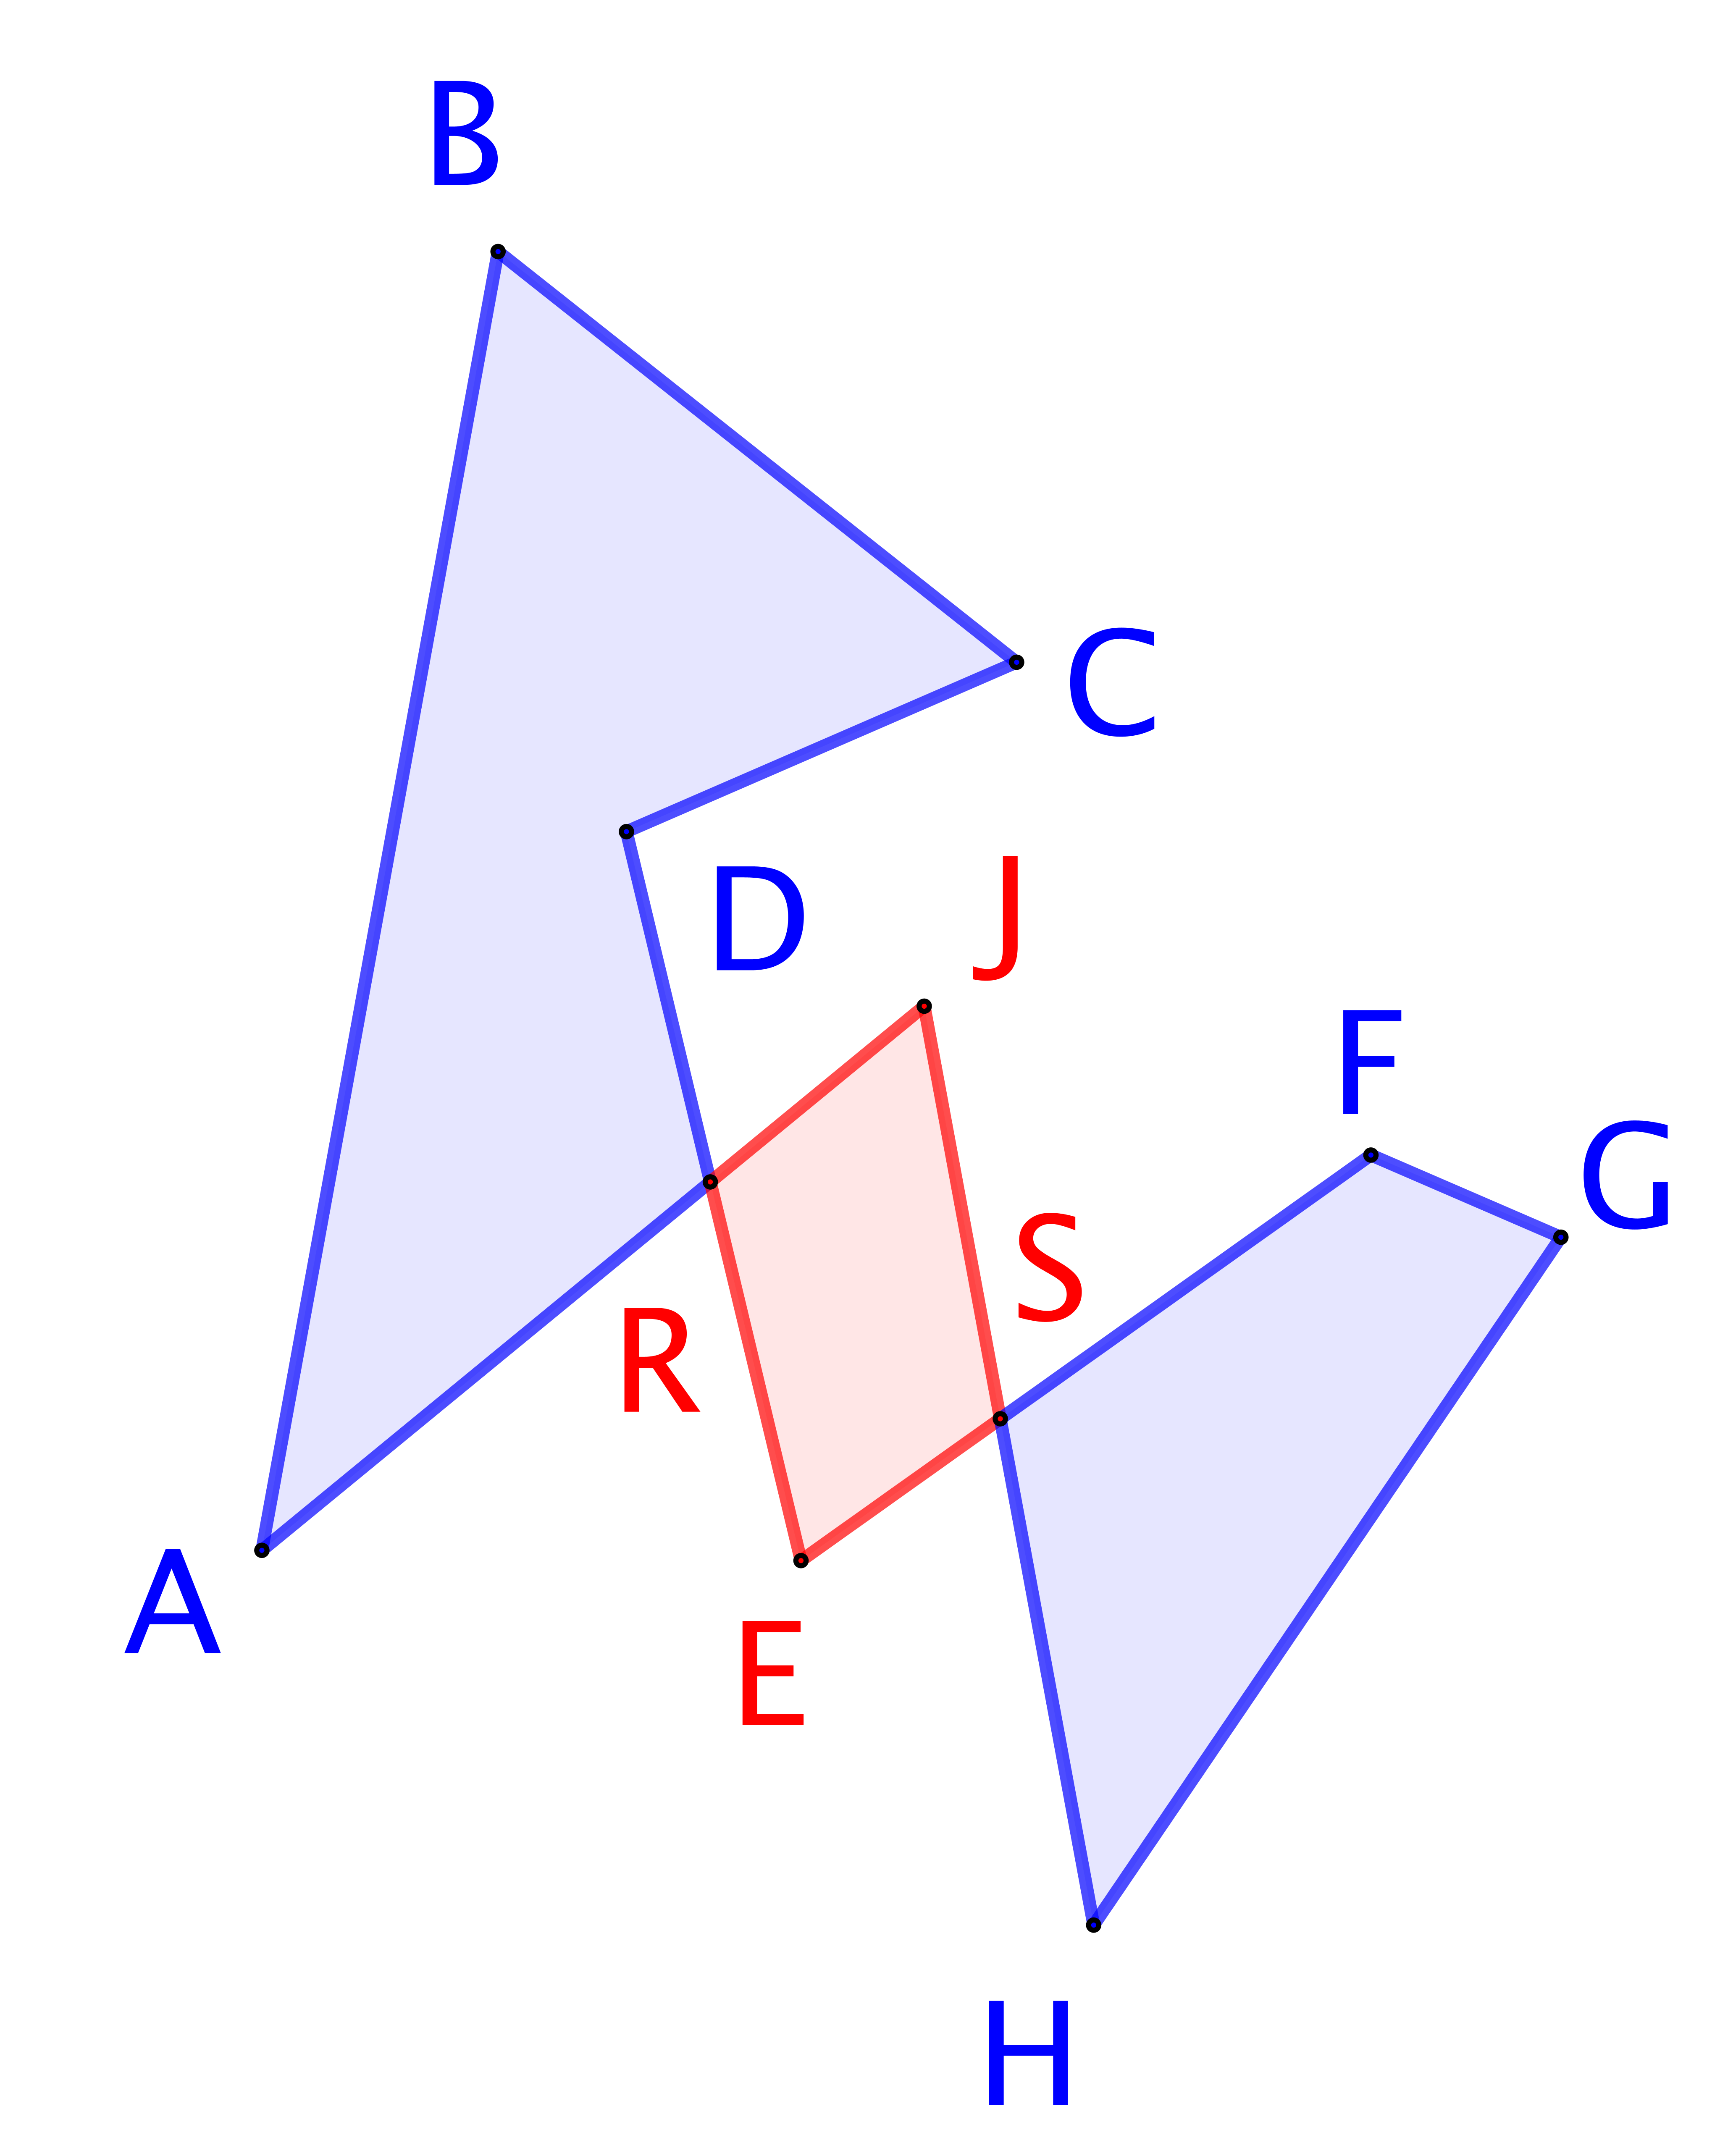
\includegraphics[scale=.35]{content/polygon/at-least-one/garea-trick.png}
\end{center}


Pour calculer l'aire généralisée d'un polygone croisé associé au \ncycle\ $\setproba{L}$, il suffit de procéder comme suit (cette méthode est utile pour un humain).
%
\begin{itemize}
    \item On part du 1\iere\ sommet de $\setproba{L}$, puis on parcourt $\setproba{L}$ dans un sens donné jusqu'à la première intersection de deux arêtes non contigües. Dans notre exemple, on va de $A$ à $R$.


    \item De cette intersection, on part en changeant de direction pour choisir celle allant vers notre point de départ. Dans notre exemple, nous obtenons le \xcycle{5} $RABCD$.


    \item Le reste des points non parcourus, en respectant le sens de parcourt initial, fournit un autre \kcycle\ qui est $REFGHI$ dans notre cas. Formellement, nous avons scindé $ABCDEFGHI$ en $RABCD$ et $REFGHI$.


    \item On répète ce processus tant qu'il reste des intersections d'arêtes non contigües, autrement dit, tant que nous n'obtenons que des \kgones.
    Pour notre exemple, il reste $REFGHI$ qui se scinde en $SIRE$ et $SFGH$.


    \item Les deux cas précédents peuvent s'écrire comme suit où l'opération \og \emph{point} \fg\ sera définie proprement plus tard (ici on peut la voir comme une forme de concaténation pointée).

    \smallskip
    \noindent\kern-1.75ex
    \begin{stepcalc}[style=ar*]
    	ABCDEFGHI
	\explnext*{Insertion de l'intersection $R$.}{}
		ABCDR \cdot REFGHI
	\explnext*{Insertion de l'intersection $S$.}{}
		ABCDR \cdot RESI \cdot SFGH
    \end{stepcalc}

    \smallskip
    \noindent
    En permutant les sommets sans changer le sens de parcours, nous retrouvons la décomposition précédente $RABCD$, $SIRE$ et $SFGH$.


    \item Ce qui précède motive les calculs suivants où $\mu(\Omega ; \setproba{L})$ indique que $\Omega$ est le point de calcul de $\mu(\setproba{L})$. Ne pas hésiter à s'aider du dessin ici.

    \smallskip
    
    \noindent\kern-1.75ex
    \begin{stepcalc}[style=ar*]
    	\mu(ABCDEFGHI)
	\explnext*{$R$ entre dans la danse.}{}
    	\mu(R ; ABCDEFGHI)
	\explnext*{$D$, $R$ et $E$ alignés, ainsi que $A$, $R$ et $I$.}{}
    	\mu(R ; ABCDR) + \mu(R ; REFGHI)
	\explnext*{$S$ est utile, lui aussi.}{}
    	\mu(ABCDR) + \mu(S ; REFGHI)
	\explnext*{$E$, $S$ et $F$ alignés, ainsi que $I$, $S$ et $H$.}{}
    	\mu(ABCDR) + \mu(S ; RESI) + \mu(S ; SFGH)
	\explnext{}
    	\mu(ABCDR) + \mu(RESI) + \mu(SFGH)
    \end{stepcalc}
    
    \smallskip
    \noindent
    Finalement,
    $\mu(ABCDEFGHI) = \area{ABCDR} - \area{RESI} + \area{SFGH}$
    selon les faits \ref{route-direction} et \ref{ngone-garea-is-area}.
    Ceci justifie $\num{6.88} - \num{2.63} + \num{4.95} = \num{9.2}$ indiqué plus haut.


    \item Il est important de noter dans les calculs précédents que pour chaque intersection utilisée pour \og \emph{éclater} \fg\ les calculs intermédiaires de $\mu(\setproba{L})$, nous avons un changement de sens de parcours du point de vue de ce point d'intersection, ceci faisant apparaître des changements de signes des aires algébriques des \ngones\ finaux.
\end{itemize}

Pour fixer mieux le mécanisme de calcul, plus combinatoire que géométrique, nous proposons l'exemple ci-après qui aboutit à $\num{12.26} - \num{1.96} = \num{10.3}$ comme attendu.%
\footnote{
	Les valeurs numériques ont été fournies par \geogebra.
}

%\newpage

\begin{multicols}{2}
	\foreach \n in {1,3,2,4} {
		\begin{center}
    		\includegraphics[scale=.35]{content/polygon/at-least-one/garea-trick-bis-\n.png}
		\end{center}
	}
\end{multicols}


% ----------------------- %


Pour une preuve formelle de ce qui précède, nous aurons besoin d'un peu de vocabulaire.


\begin{defi}
    Soient
    $\setproba{L} = A_1 A_2 \cdots A_n$ 
    et
    $\setproba{L}^{\,\prime} = B_1 B_2 \cdots B_k$ 
    deux cycles.
    %
    Leur \og \emph{unification} \fg\ est le \xcycle{(n+k)} $\setproba{L} \cdot \setproba{L}^{\,\prime} = A_1 A_2 \cdots A_n B_1 B_2 \cdots B_k$.
    Clairement, $\setproba{L} \cdot \setproba{L}^{\,\prime} = \setproba{L}^{\,\prime} \cdot \setproba{L}$.
\end{defi}


Cette notion d'unification n'est pas toujours pertinente comme le montre l'exemple suivant, mais nous n'unifierons que dans le cadre très particulier des intersections d'arêtes non contigües d'un \ncycle.


\begin{multicols}{2}
    \small\itshape
    \begin{center}
        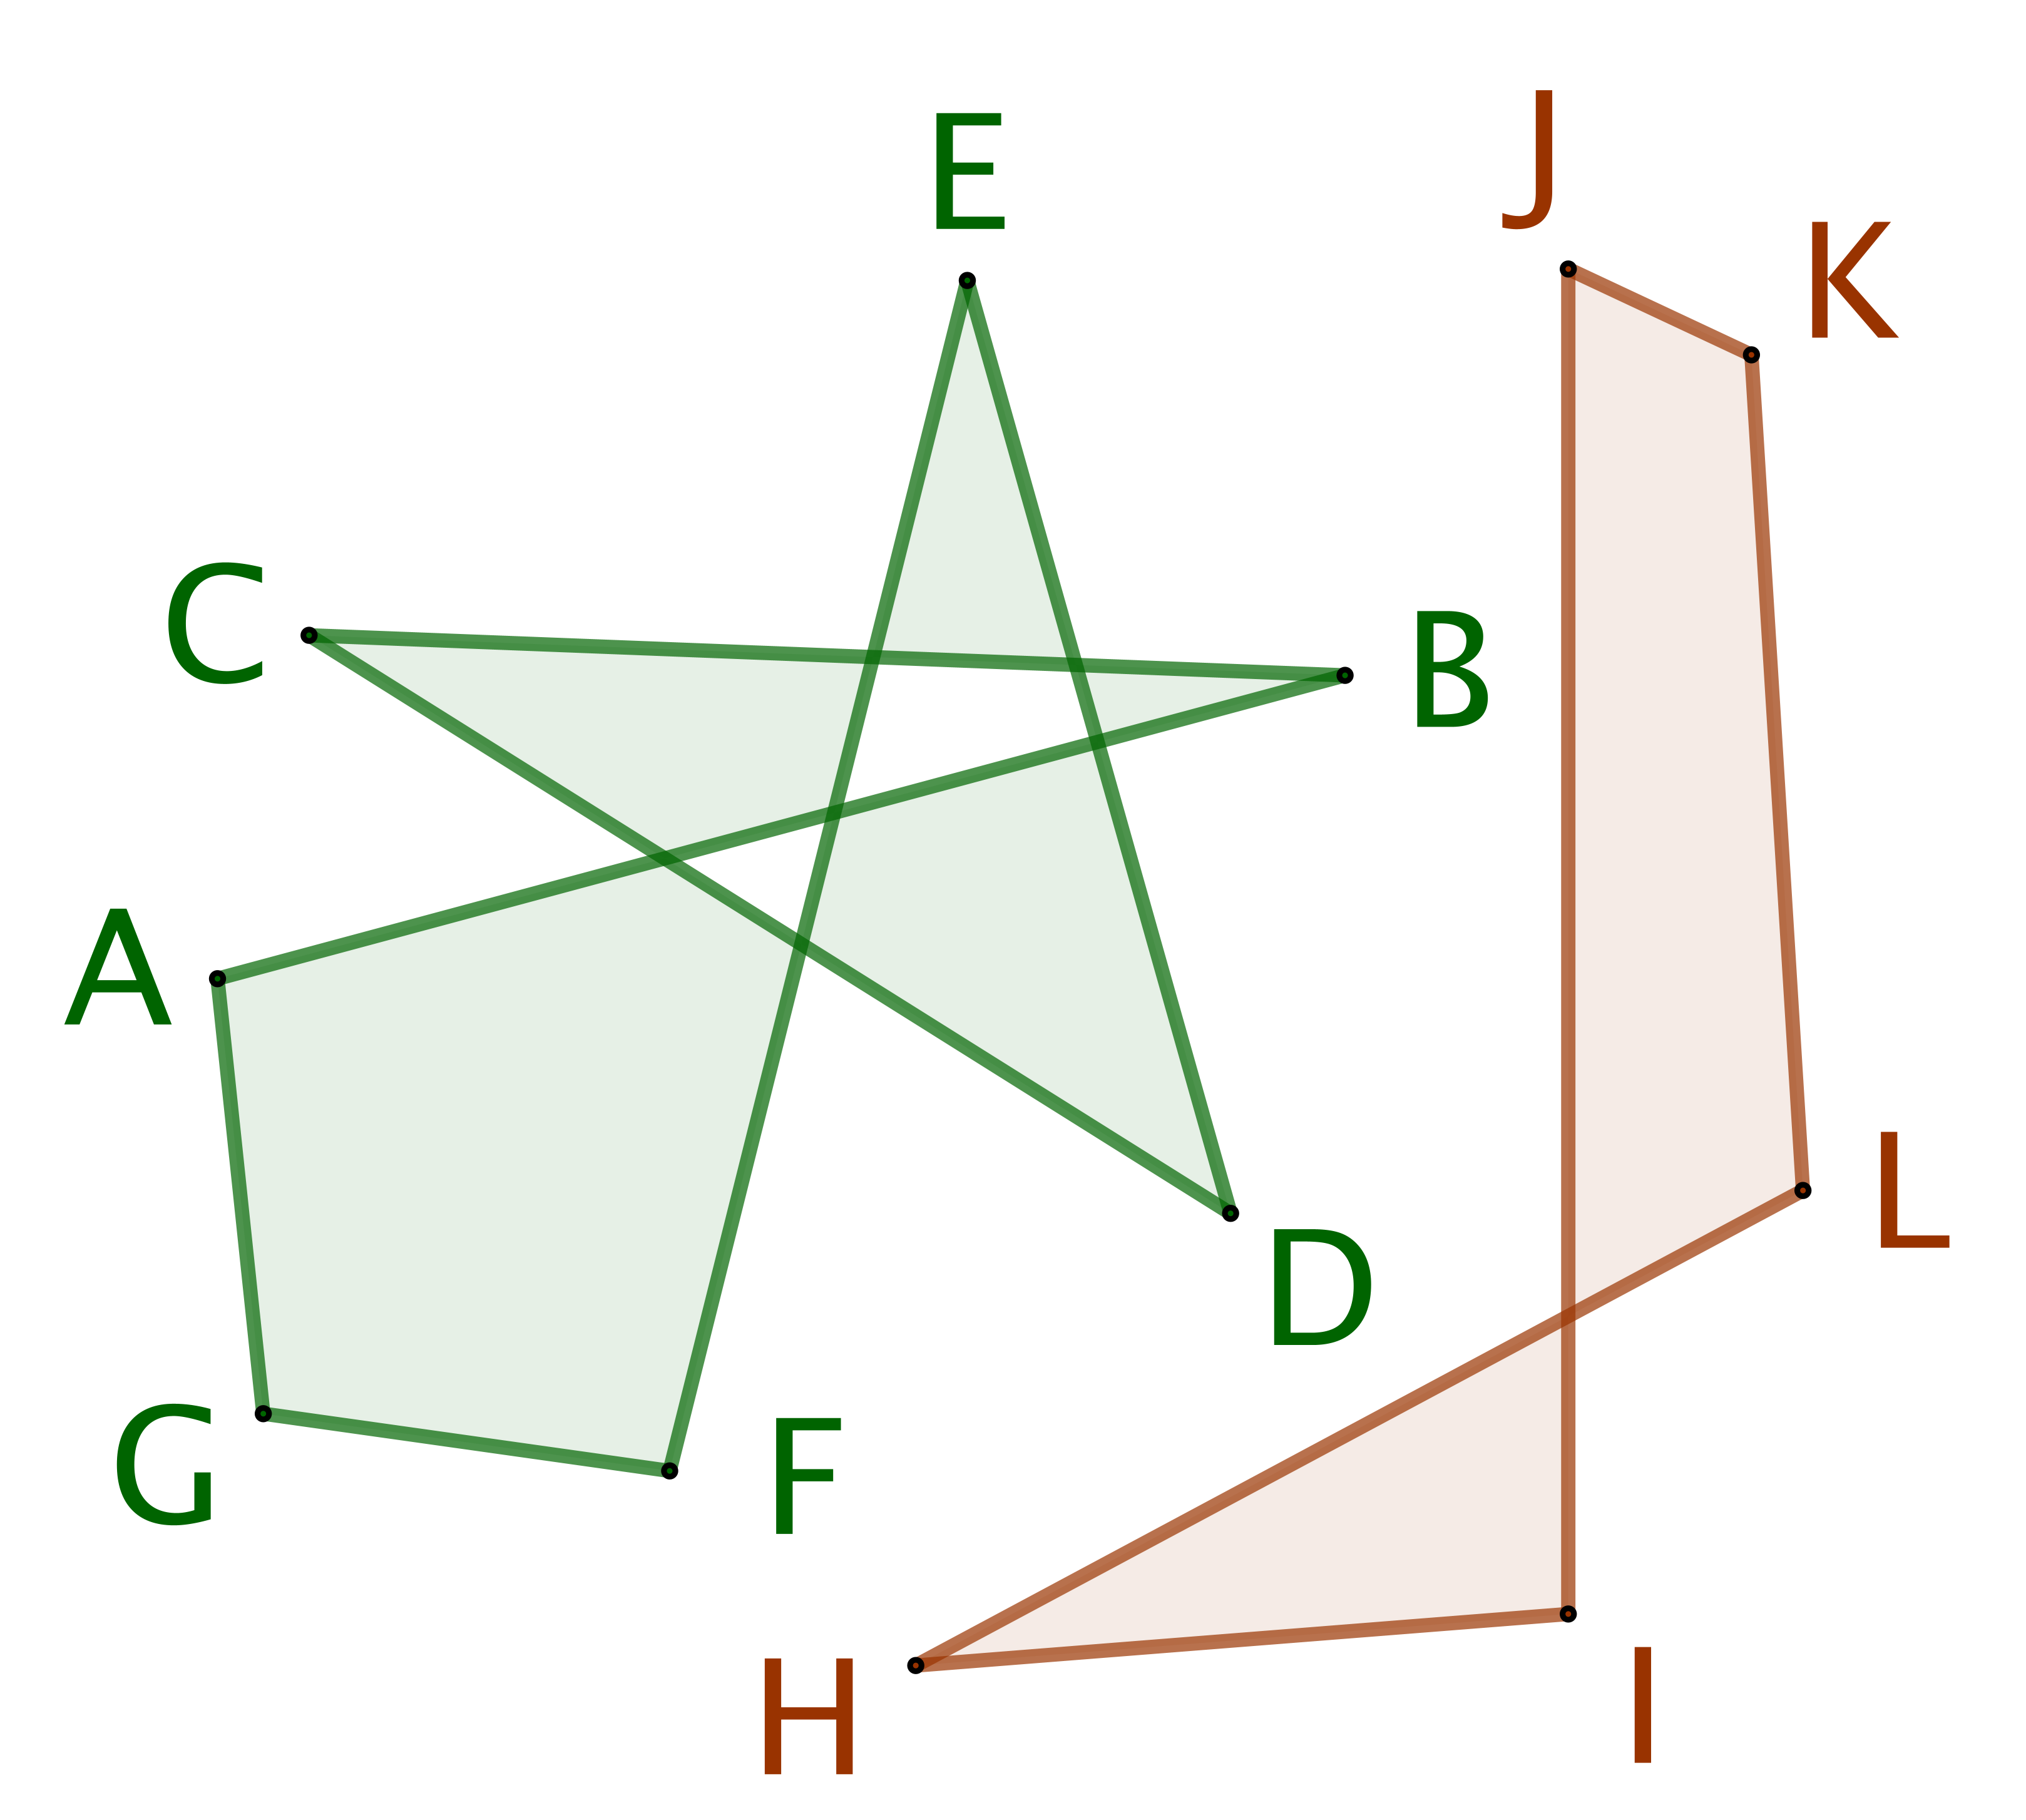
\includegraphics[scale=.4]{content/polygon/at-least-one/unification-1.png}

        \smallskip
        Deux cycles libres.
    \end{center}


    \begin{center}
        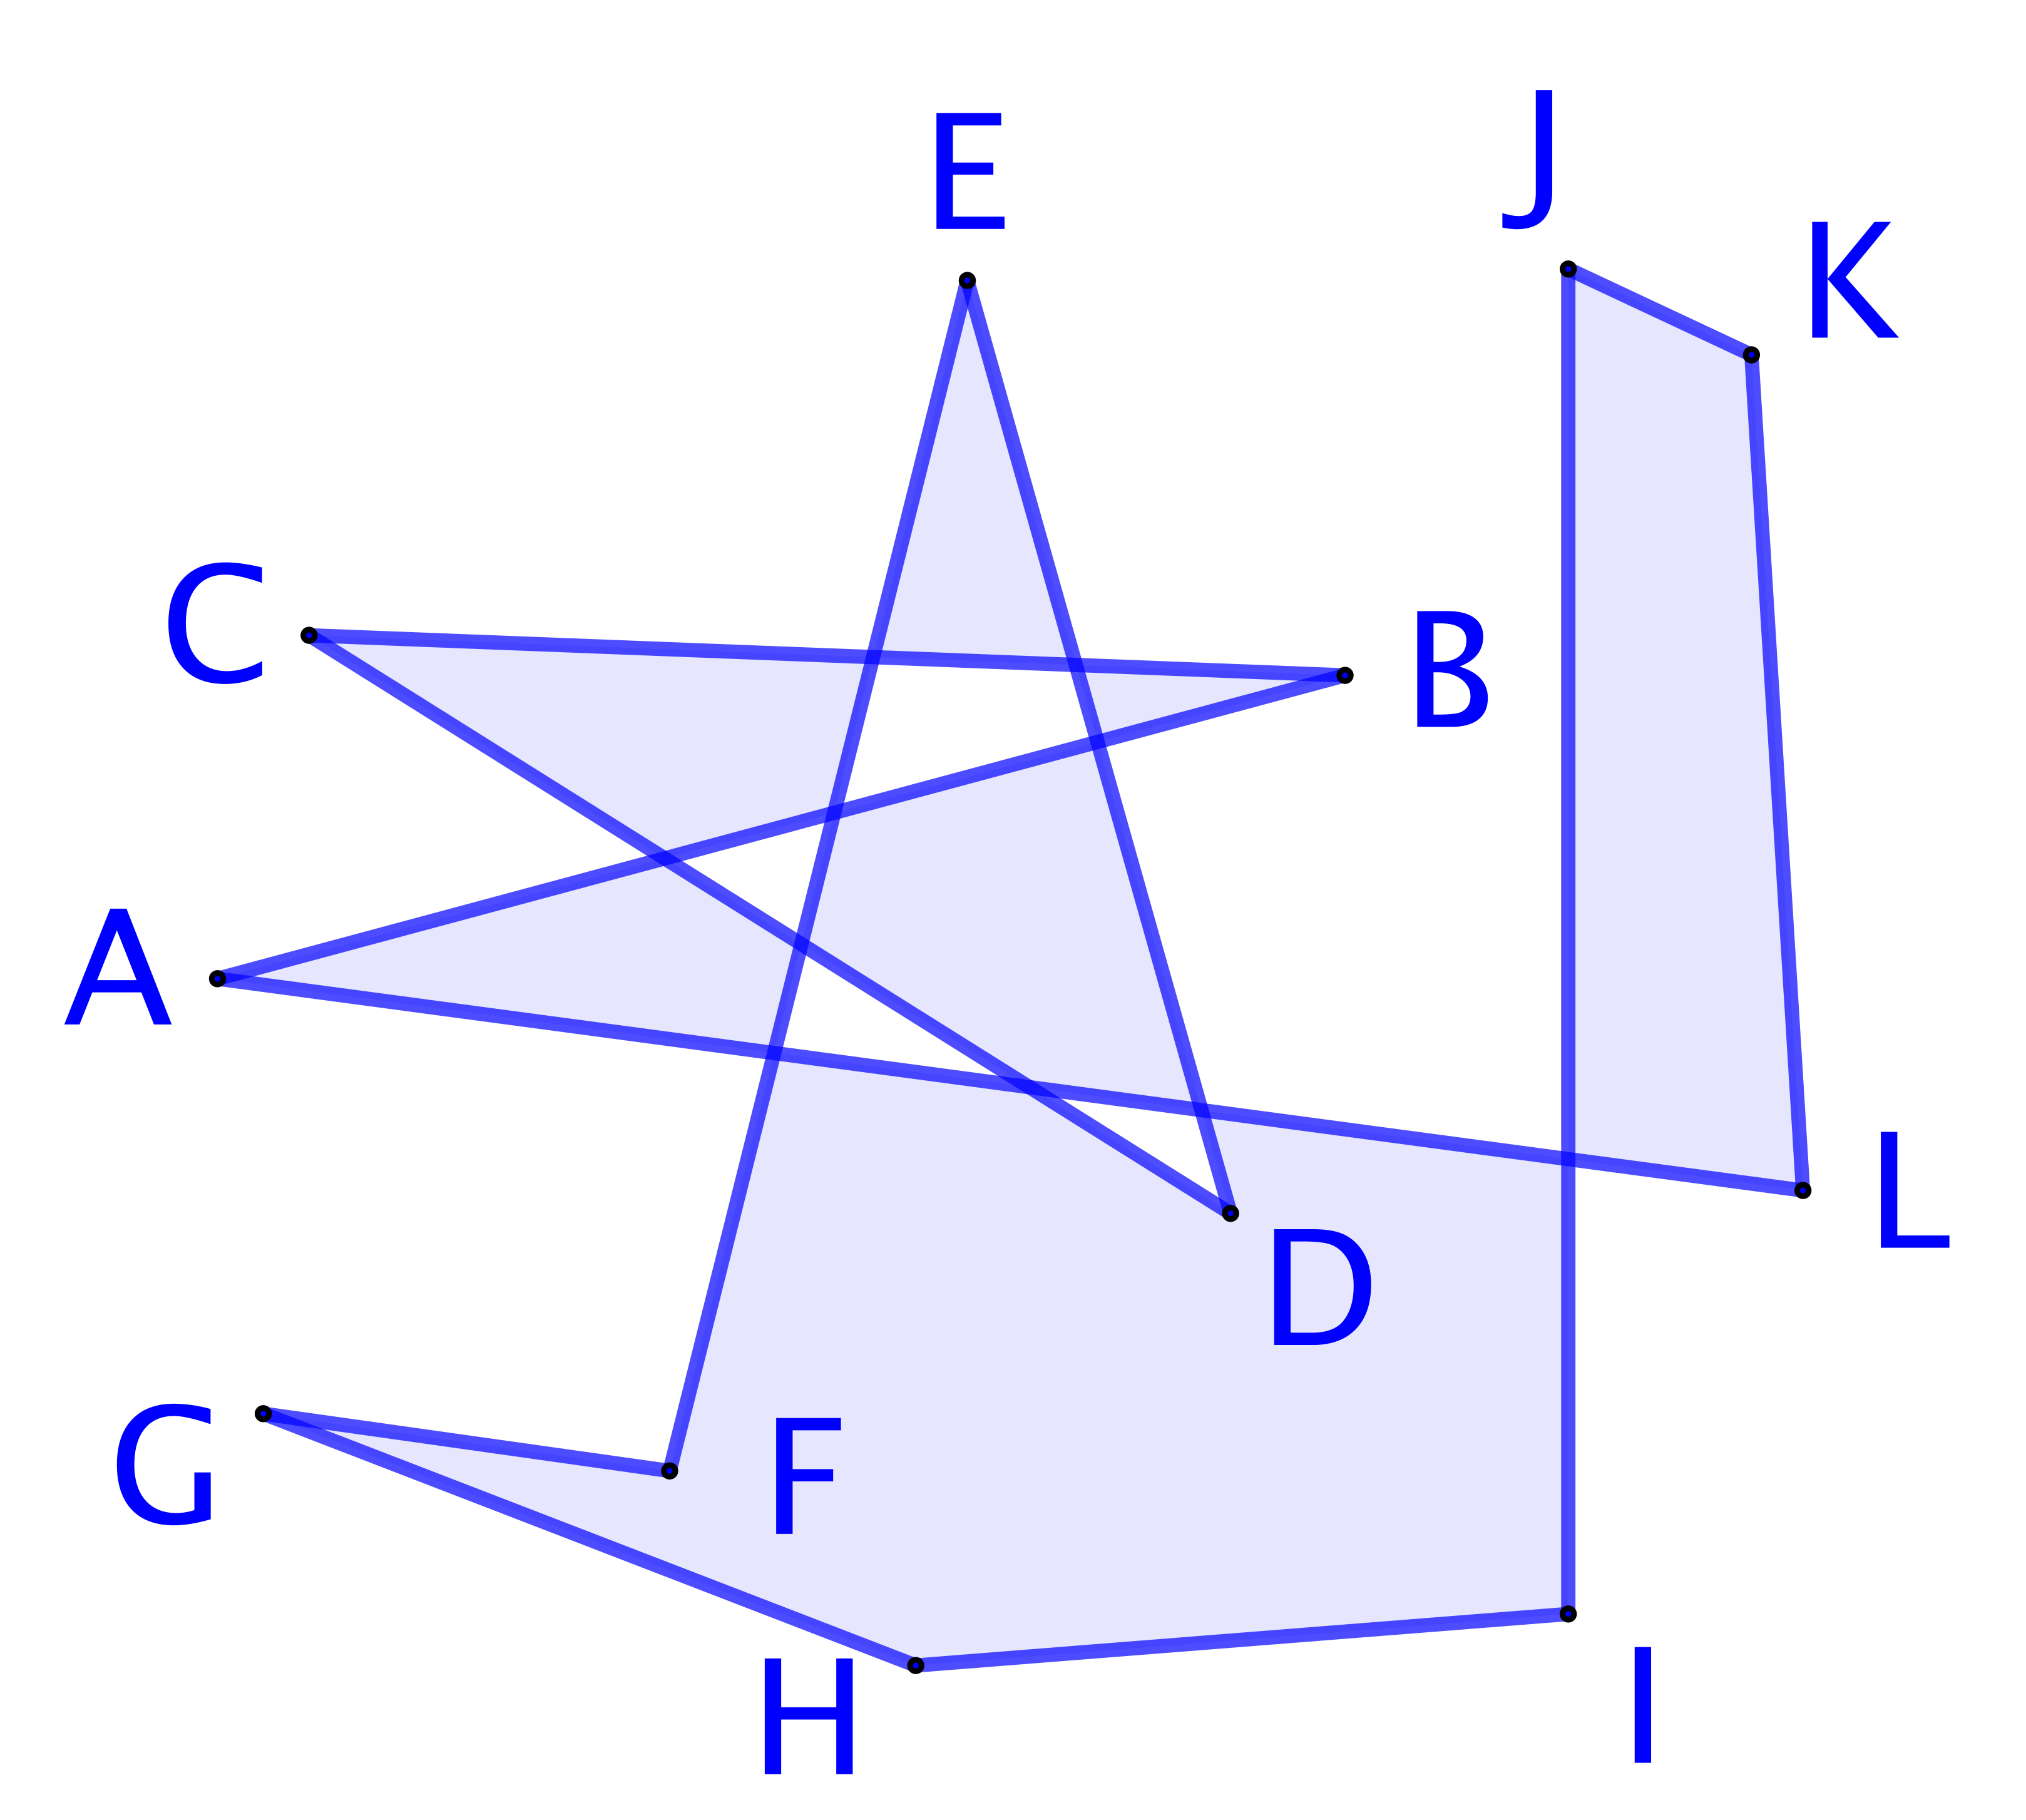
\includegraphics[scale=.4]{content/polygon/at-least-one/unification-2.png}

        \smallskip
        Deux cycles unifiés.
    \end{center}
\end{multicols}


% ----------------------- %


\begin{defi}
    Deux cycles
    $\setproba{L} = A_1 A_2 \cdots A_n$ 
    et
    $\setproba{L}^{\,\prime} = B_1 B_2 \cdots B_k$ 
    sont \og \emph{mariables} \fg\ lorsque
    $B_1 \in [B_k A_2]$,
    $A_1 \in [A_n B_2]$
    et
    $A_1 = B_1$.
\end{defi}


L'exemple suivant montre que l'unification de deux cycles mariables est paisible.%
\footnote{
	L'histoire ne dit pas s'il en va de même pour les hommes.
}

\begin{multicols}{2}
    \small\itshape
    \begin{center}
        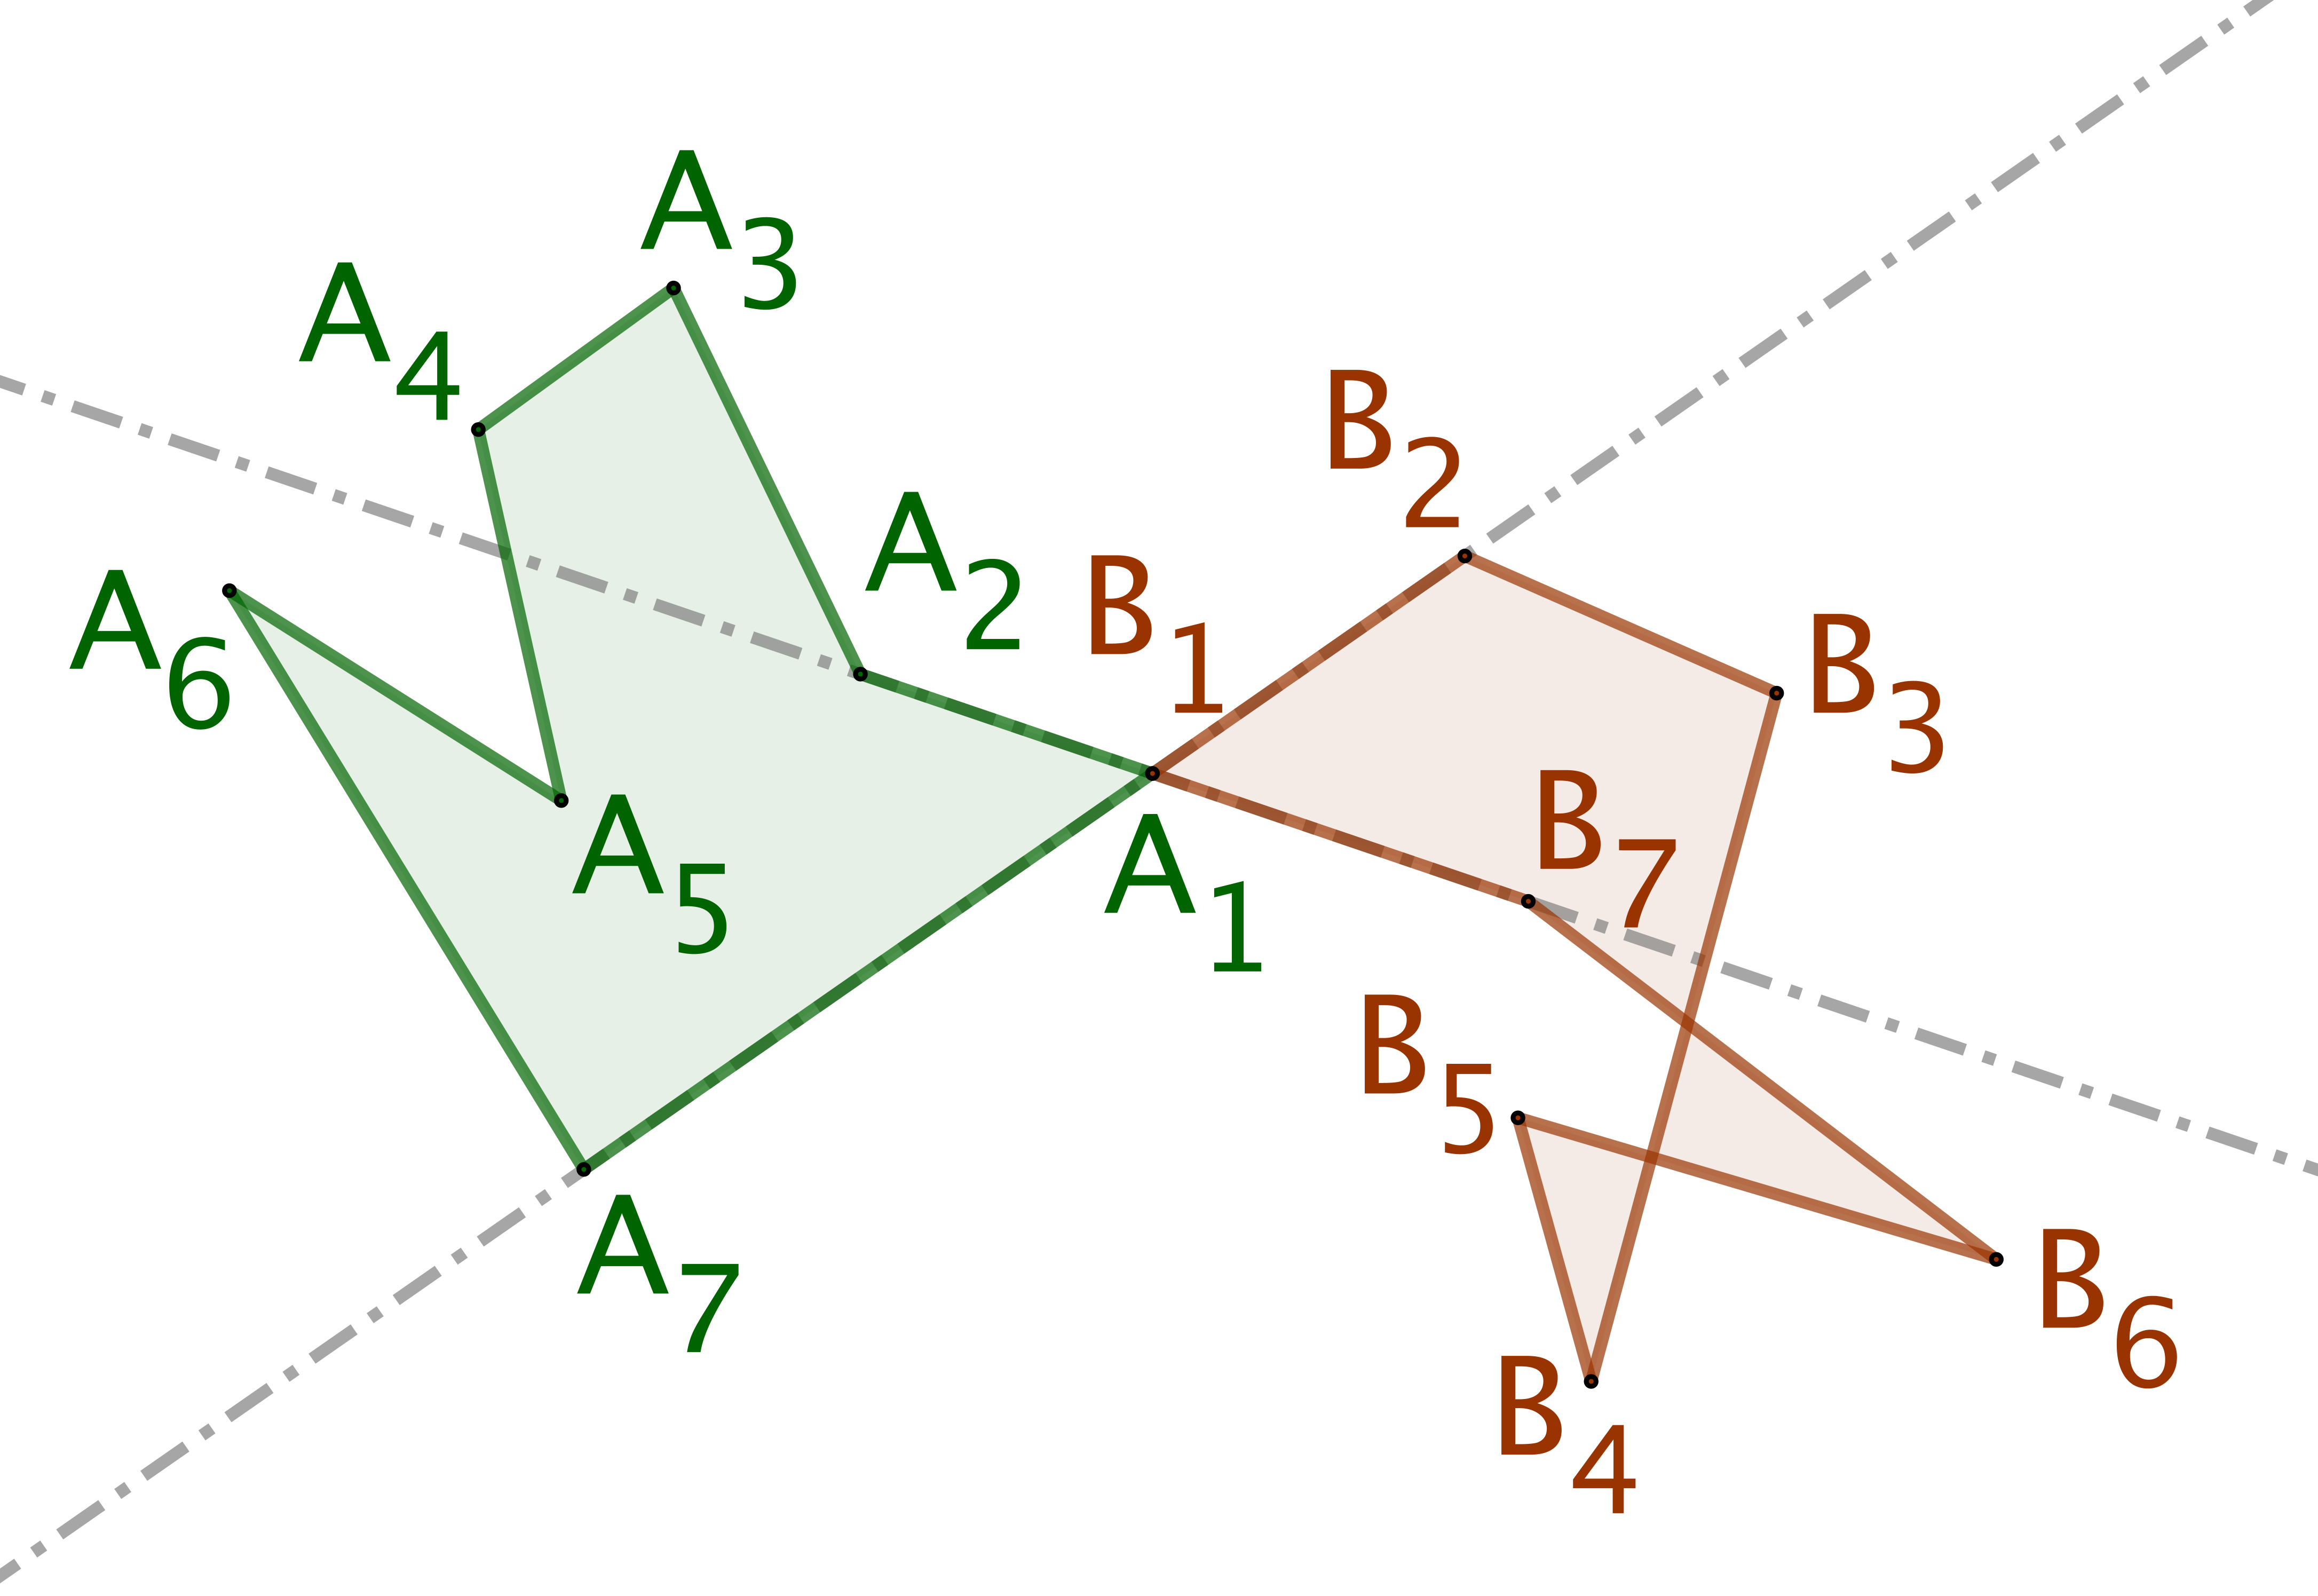
\includegraphics[scale=.4]{content/polygon/at-least-one/wedding-1.png}

        \smallskip
        Deux cycles mariables.
    \end{center}


    \begin{center}
        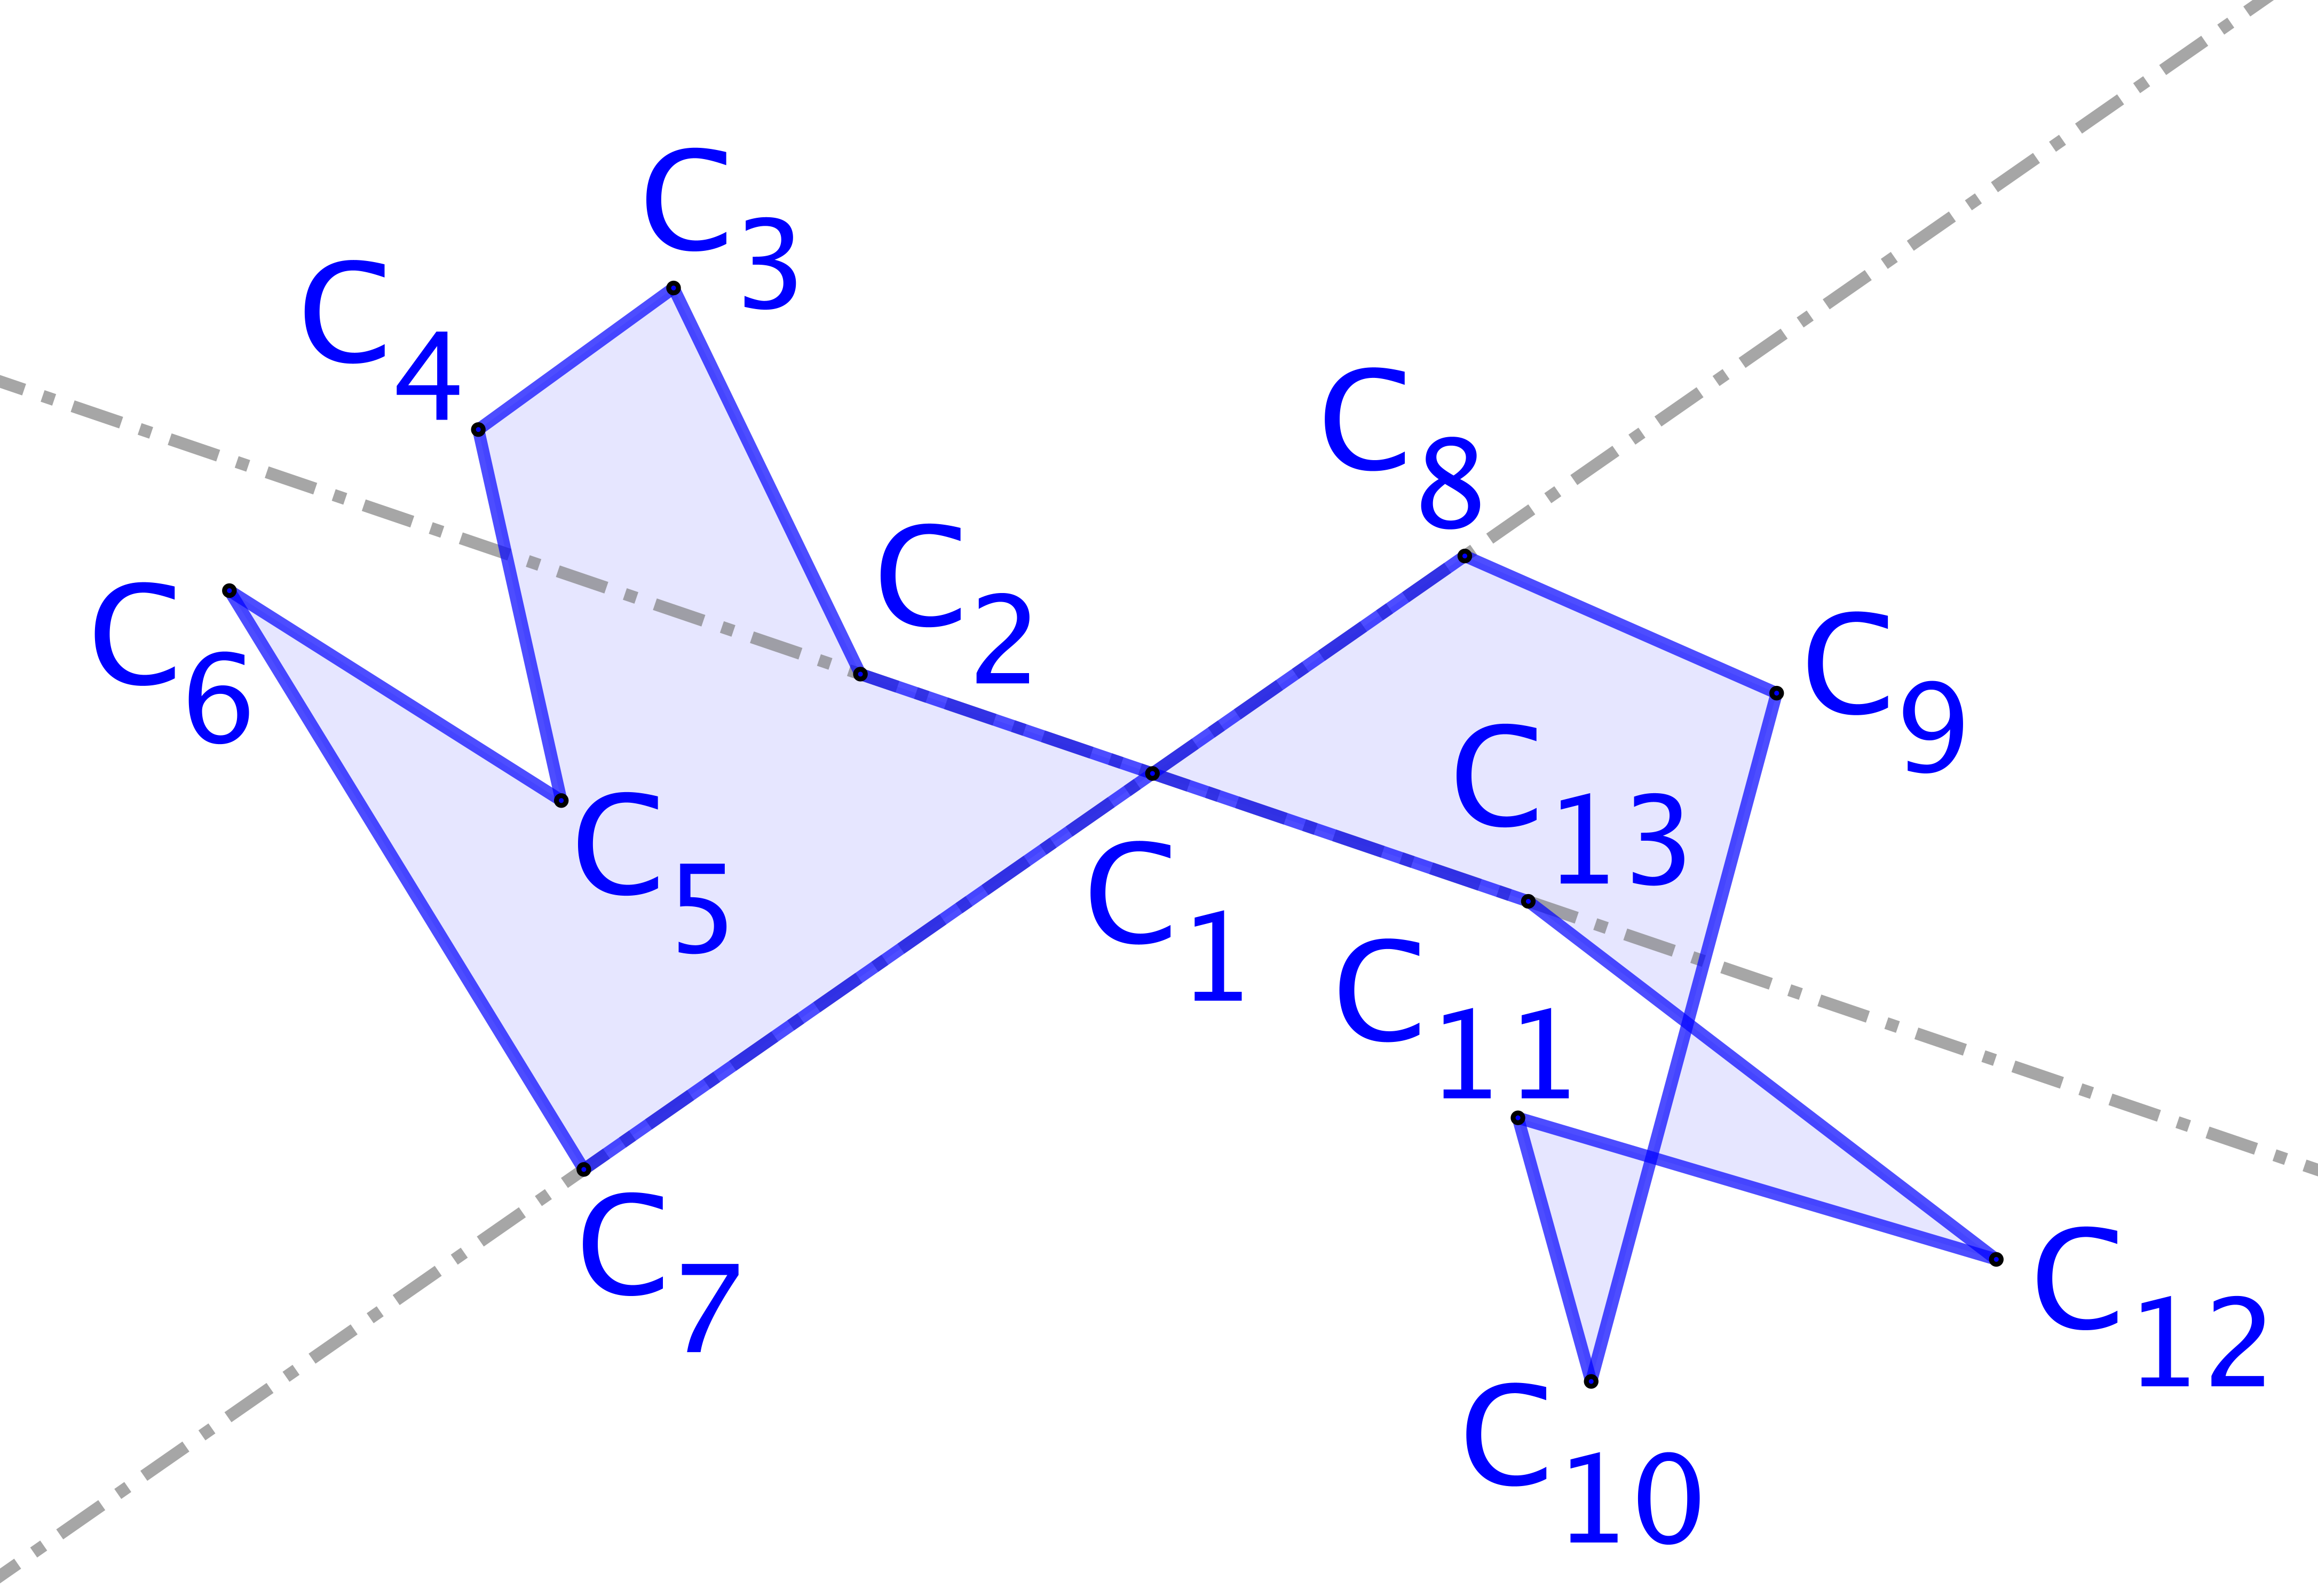
\includegraphics[scale=.4]{content/polygon/at-least-one/wedding-2.png}

        \smallskip
        Deux cycles dans le rang.
    \end{center}
\end{multicols}
    
    
% ----------------------- %


\begin{fact} \label{nline-pseudo-chasles}
    Si les cycles
    $\setproba{L} = A_1 A_2 \cdots A_n$
    et
    $\setproba{L}^{\,\prime} = B_1 B_2 \cdots B_k$
    vérifient $A_1 = B_1$, alors nous avons
    $ \mu( \setproba{L} \cdot \setproba{L}^{\,\prime} )
    = \mu( \setproba{L} ) + \mu( \setproba{L}^{\,\prime} )$.
\end{fact}


\begin{proof}
	Ci-dessous, $\mu(\Omega ; \setproba{L})$ indique que $\Omega$ est le point de calcul de $\mu(\setproba{L})$.

    \smallskip
    
    \noindent\kern-1.75ex
    \begin{stepcalc}[style=ar*]
    	\mu( \setproba{L} \cdot \setproba{L}^{\,\prime} )
	\explnext{}
    	\mu(A_1 ; \setproba{L} \cdot \setproba{L}^{\,\prime})
	\explnext{}
    	\dsum_{j=1}^{n-1}
			\det \big( \vect{A_1 A_j} , \vect{A_1 A_{j + 1}} \big)
    	+
	    	\det \big( \vect{A_1 A_n} , \vect{A_1 B_1} \big)
    	+
	    \dsum_{j=1}^{k-1}
			\det \big( \vect{A_1 B_j} , \vect{A_1 B_{j + 1}} \big)
    	+
	    	\det \big( \vect{A_1 B_k} , \vect{A_1 A_1} \big)
	\explnext{}
    	\dsum_{j=1}^{n-1}
			\det \big( \vect{A_1 A_j} , \vect{A_1 A_{j + 1}} \big)
    	+
	    \dsum_{j=1}^{k-1}
			\det \big( \vect{A_1 B_j} , \vect{A_1 B_{j + 1}} \big)
	\explnext*{$A_1 = B_1$
	        \\ $A^{\,\prime}_{n+1} = A_1$
	        \\ $B^{\,\prime}_{k+1} = B_1$}{}
    	\dsum_{j=1}^{n}
			\det \big( \vect{A_1 A^{\,\prime}_j} , \vect{A_1 A^{\,\prime}_{j + 1}} \big)
    	+
	    \dsum_{j=1}^{k}
			\det \big( \vect{B_1 B^{\,\prime}_j} , \vect{B_1 B^{\,\prime}_{j + 1}} \big)
	\explnext{}
    	\mu(A_1 ; \setproba{L}) + \mu(B_1 ; \setproba{L}^{\,\prime})
	\explnext{}
    	\mu(\setproba{L}) + \mu(\setproba{L}^{\,\prime})
    \end{stepcalc}

    \null\vspace{-3.5ex}
\end{proof}


% ----------------------- %


\newpage

\begin{fact} \label{ngone-trick}
    Tout \ncycle\ $\setproba{L}$ non dégénéré admet une décomposition
    $\setproba{L}_1 \cdot \setproba{L}_2 \cdot ... \cdot \setproba{L}_s$ 
    vérifiant les conditions suivantes où $s \in \NNs$.
    %
    \begin{enumerate}
    	\item $\forall i \in \ZintervalC{1}{s}$, $\setproba{L}_i$ est un \xgone{k_i}.
	
    	\item $\forall i \in \ZintervalC{1}{s-1}$, $\setproba{L}_i$ et $\setproba{L}_{i+1}$ sont mariables.

    	\item Les surfaces intérieures des \xgones{k_i} $\setproba{L}_i$ sont disjointes deux à deux.
    \end{enumerate}
    
    Pour une telle décomposition, 
    $ \garea{\setproba{L}} 
    = \abs*{\,
    	  \dsum_{j} \area{\setproba{L}_{2j + 1}}  
		- \dsum_{j} \area{\setproba{L}_{2j}}
	  \,}$.
\end{fact}


\begin{proof}
	Nommons, temporairement, \og \emph{point d'intersection} \fg\ toute intersection de deux côtés non contigüs.
	Si $\setproba{L}$ n'a aucun point d'intersection,
	le choix $\setproba{L}_1 = \setproba{L}$ avec $s = 1$ convient.
	Supposons maintenant que $\setproba{L} = A_1 A_2 \cdots A_n$ admet au moins un point d'intersection.

	\begin{center}
		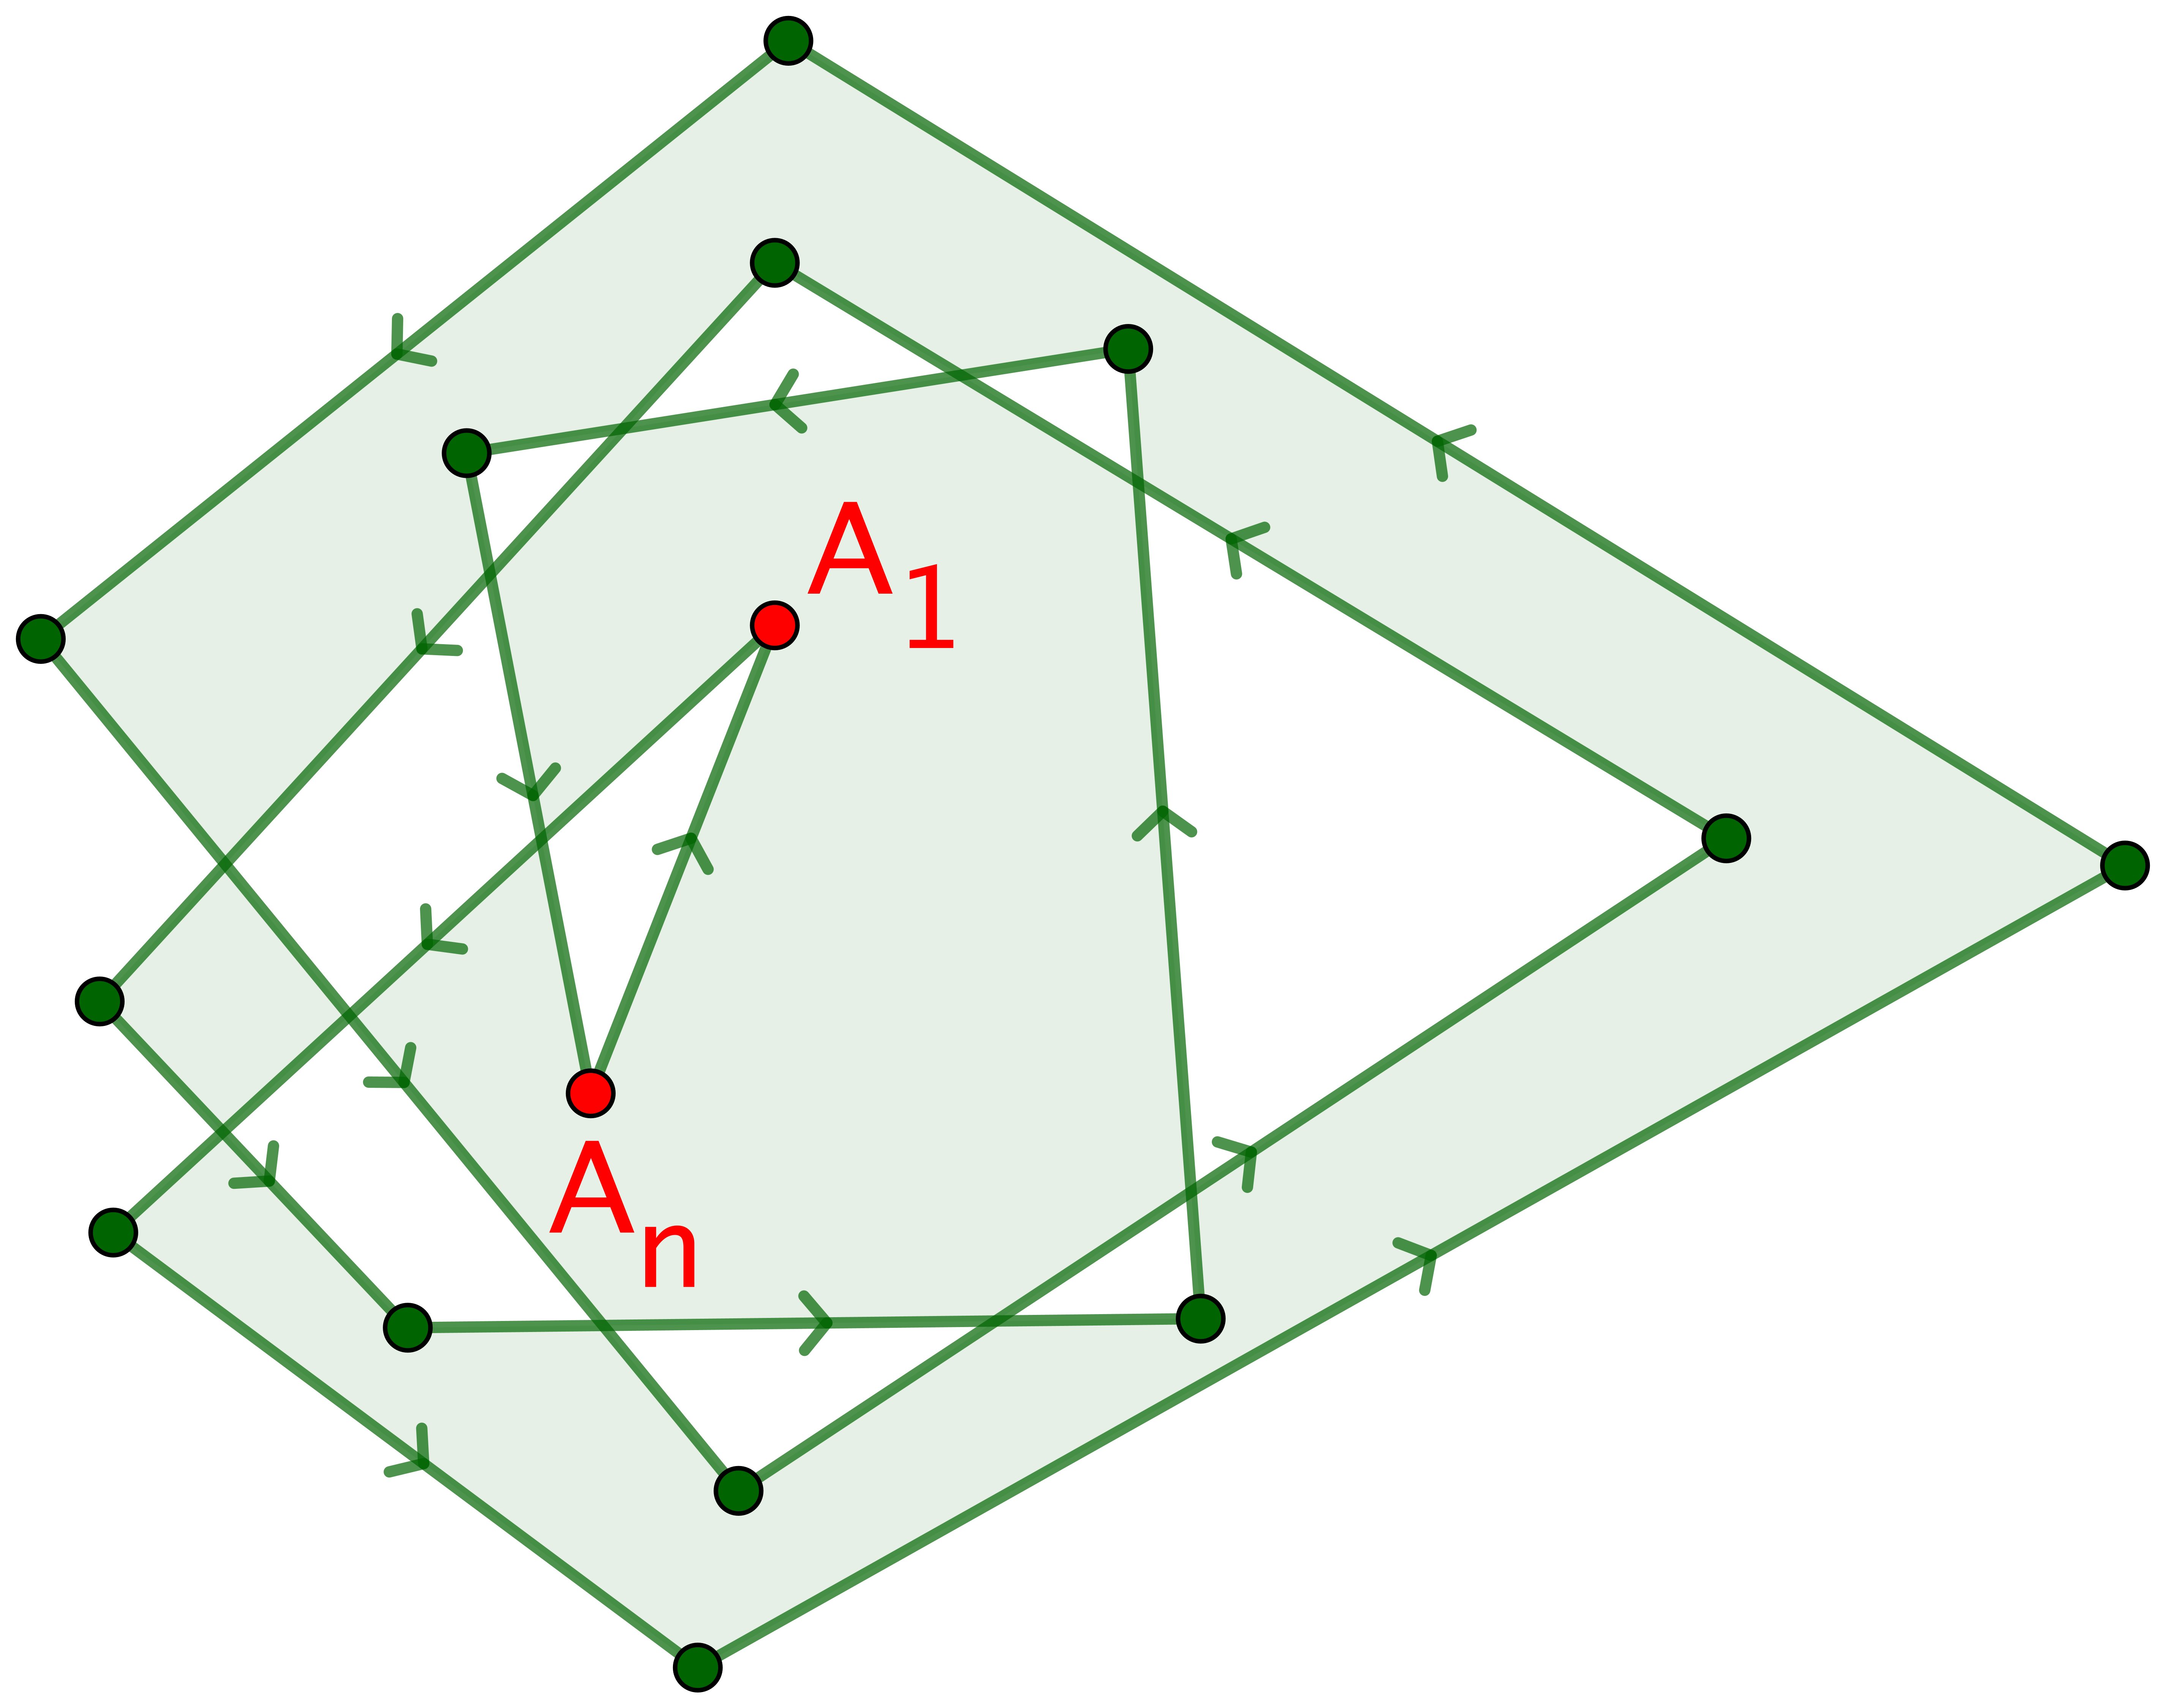
\includegraphics[scale=.35]{content/polygon/at-least-one/ngone-trick-1.png}

		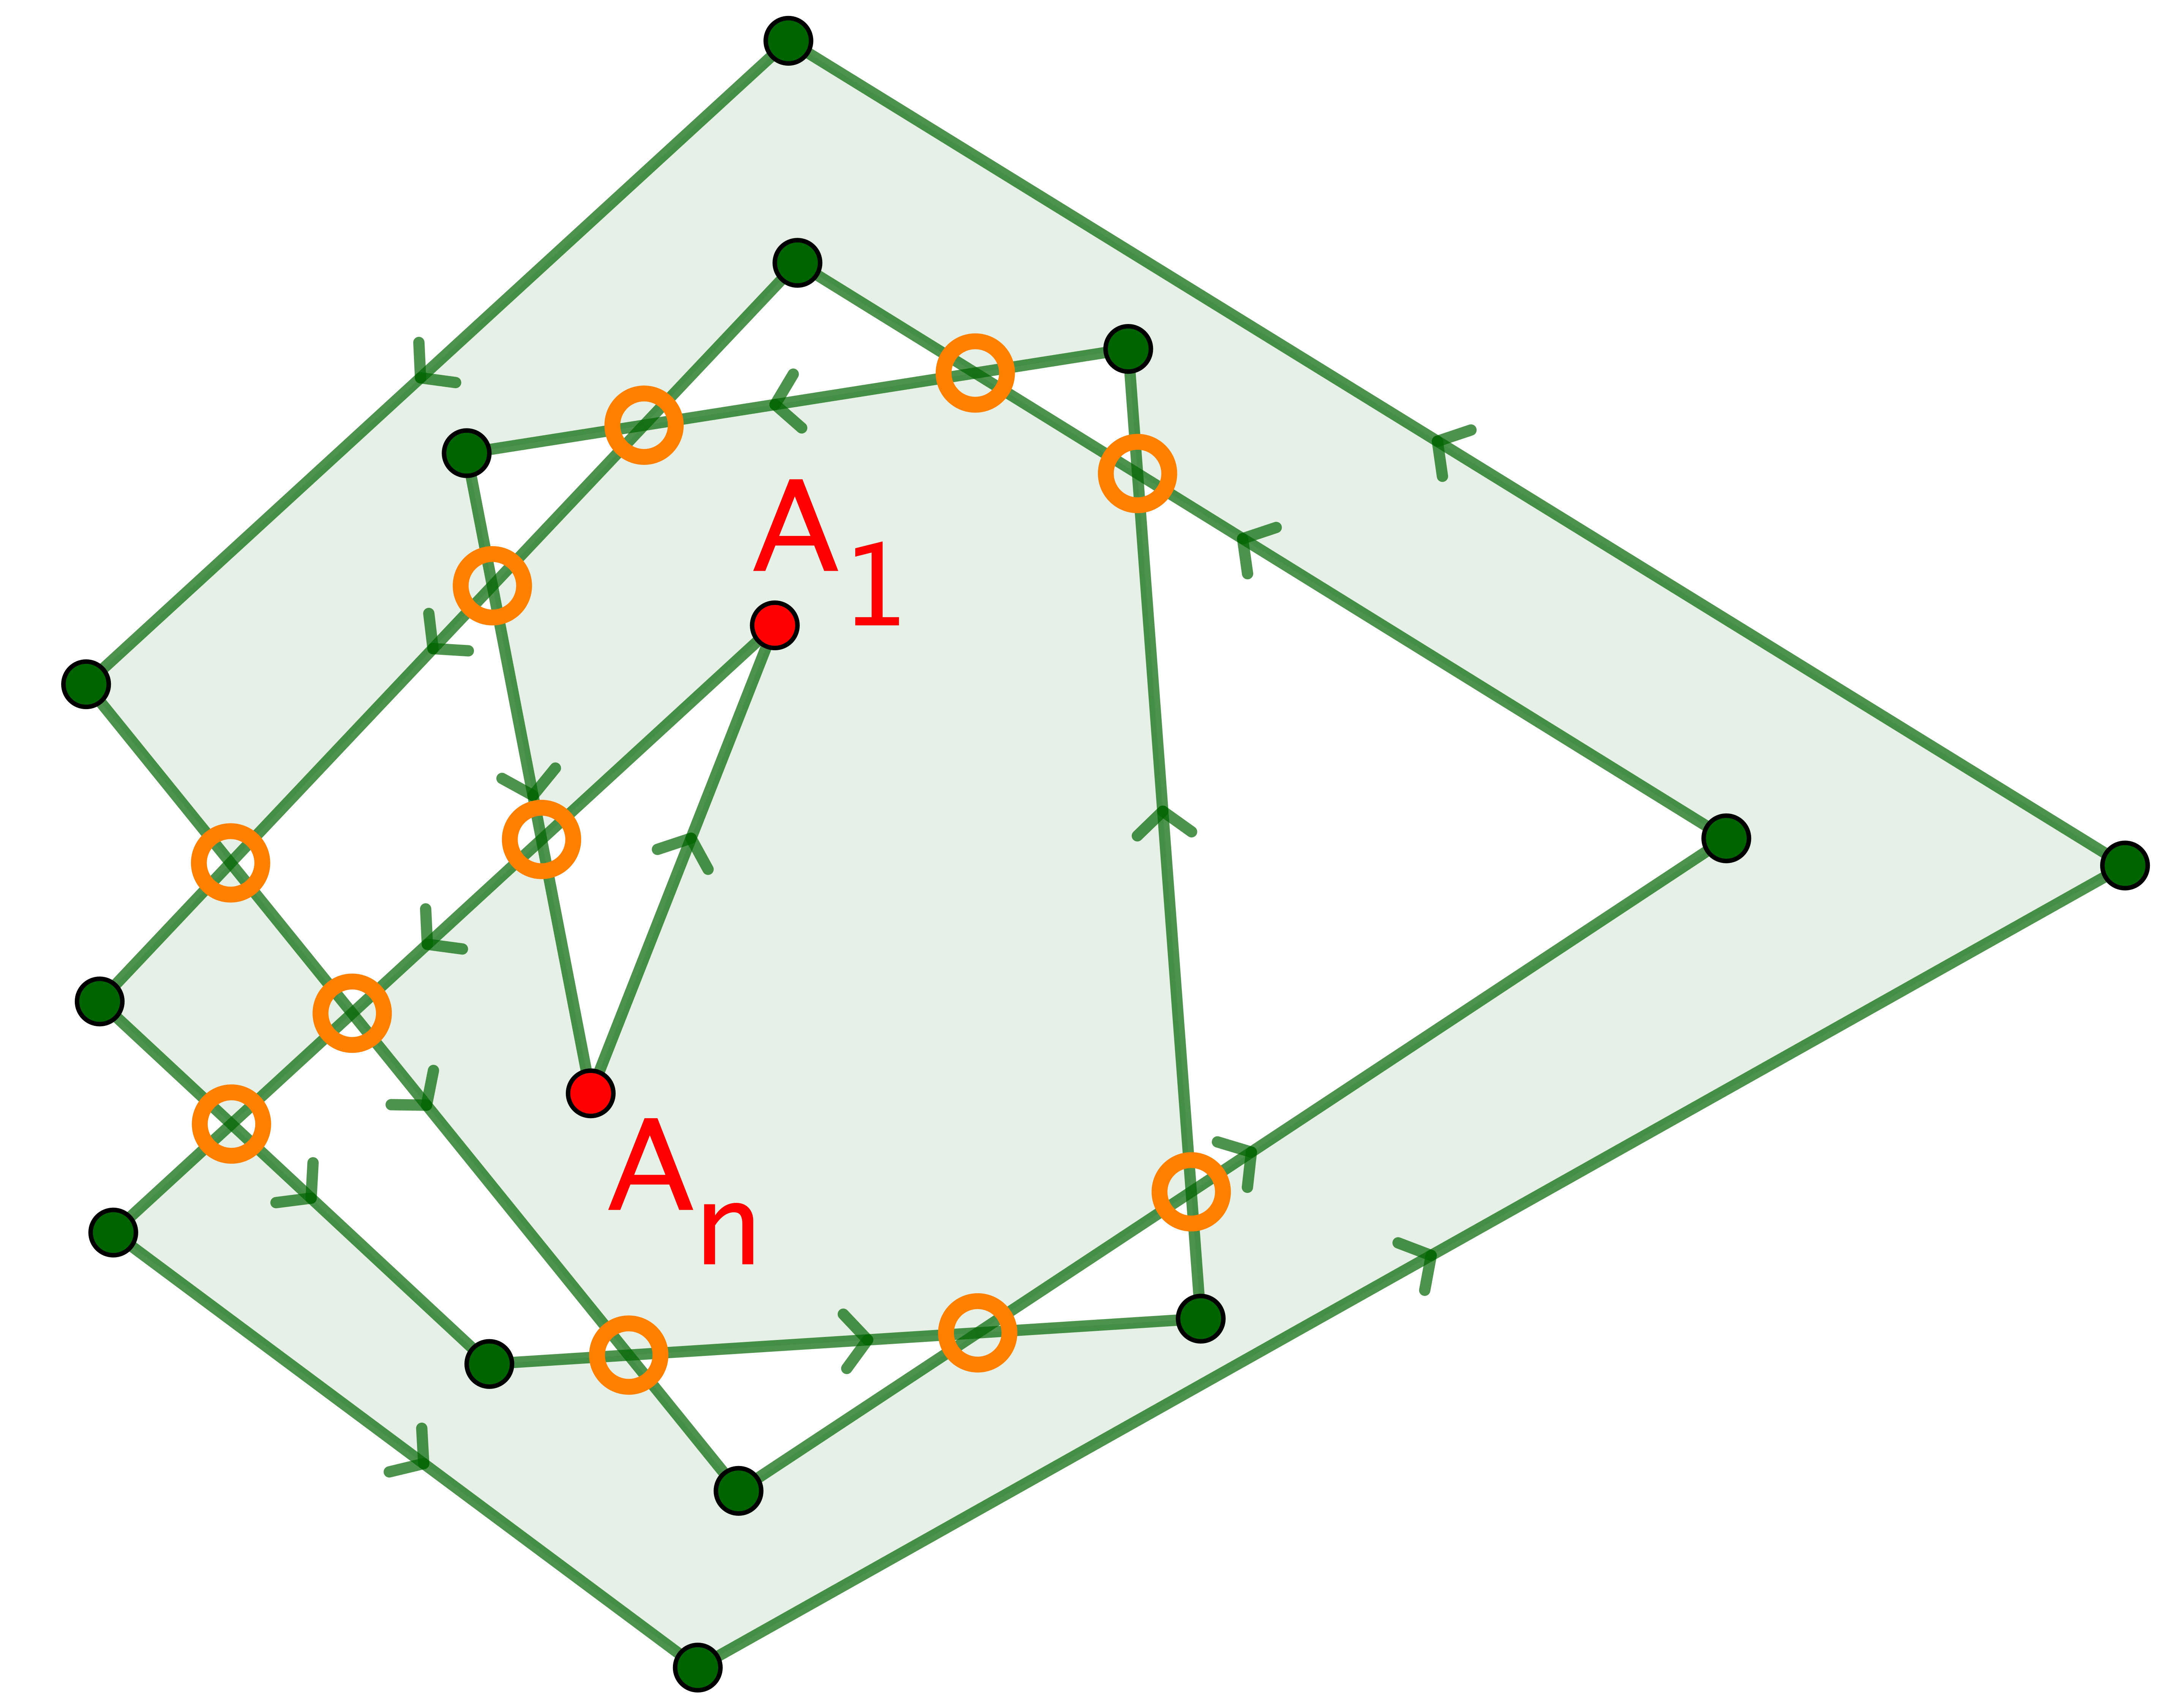
\includegraphics[scale=.35]{content/polygon/at-least-one/ngone-trick-2.png}

		\includegraphics[scale=.35]{content/polygon/at-least-one/ngone-trick-3.png}
	\end{center}


    XXX
    
    Nous pouvons faire les observations suivantes.
	%
    \begin{itemize}
    	\item 

    	\item 

    	\item 

    	\item 
    \end{itemize}
	
	
	
	 
    XXX
    
   
	Posant
	$\setproba{L}_1 = A_1 \cdots A_i I$
    et
    $\setproba{L}^{\,\prime} = I A_{i+1} \cdots A_n$,
    
    \smallskip
    
    Nous obtenons $\setproba{L} = \setproba{L}_1 \cdot \setproba{L}^{\,\prime}$ où

    avec $\setproba{L}_1$ un \ngone, car non dégénéré et sans point d'intersection.
    
    
    
\end{proof}



%% ----------------------- %
%
%
%\begin{fact} \label{no-cross-max}
%    Si un \ncycle\ $\setproba{L}$, éventuellement dégénéré, n'est pas un \ngone\ convexe, alors il existe un \ngone\ convexe $\setproba{P}$ tel que
%	$\perim{\setproba{P}} = \perim{\setproba{L}}$
%	et
%	$\garea{\setproba{P}} > \garea{\setproba{L}}$.
%\end{fact}
%
%
%\begin{proof}
%	Commençons par le cas \og hyper-dégénéré \fg: si tous les sommets de $\setproba{L}$ sont alignés, son aire généralisée est nulle. Le triangle équilatéral de côté $\frac13 \perim{\setproba{L}}$ permet de conclure.
%	%
%	Supposons maintenant qu'au moins trois sommets non alignés existent.
%	Notons $\setproba{C}$ l'enveloppe convexe de $\setproba{L}$ (nous savons que $\setproba{C}$ contient au moins un triangle).
%	
%	\begin{center}
%		\centering
%		\small\itshape
%		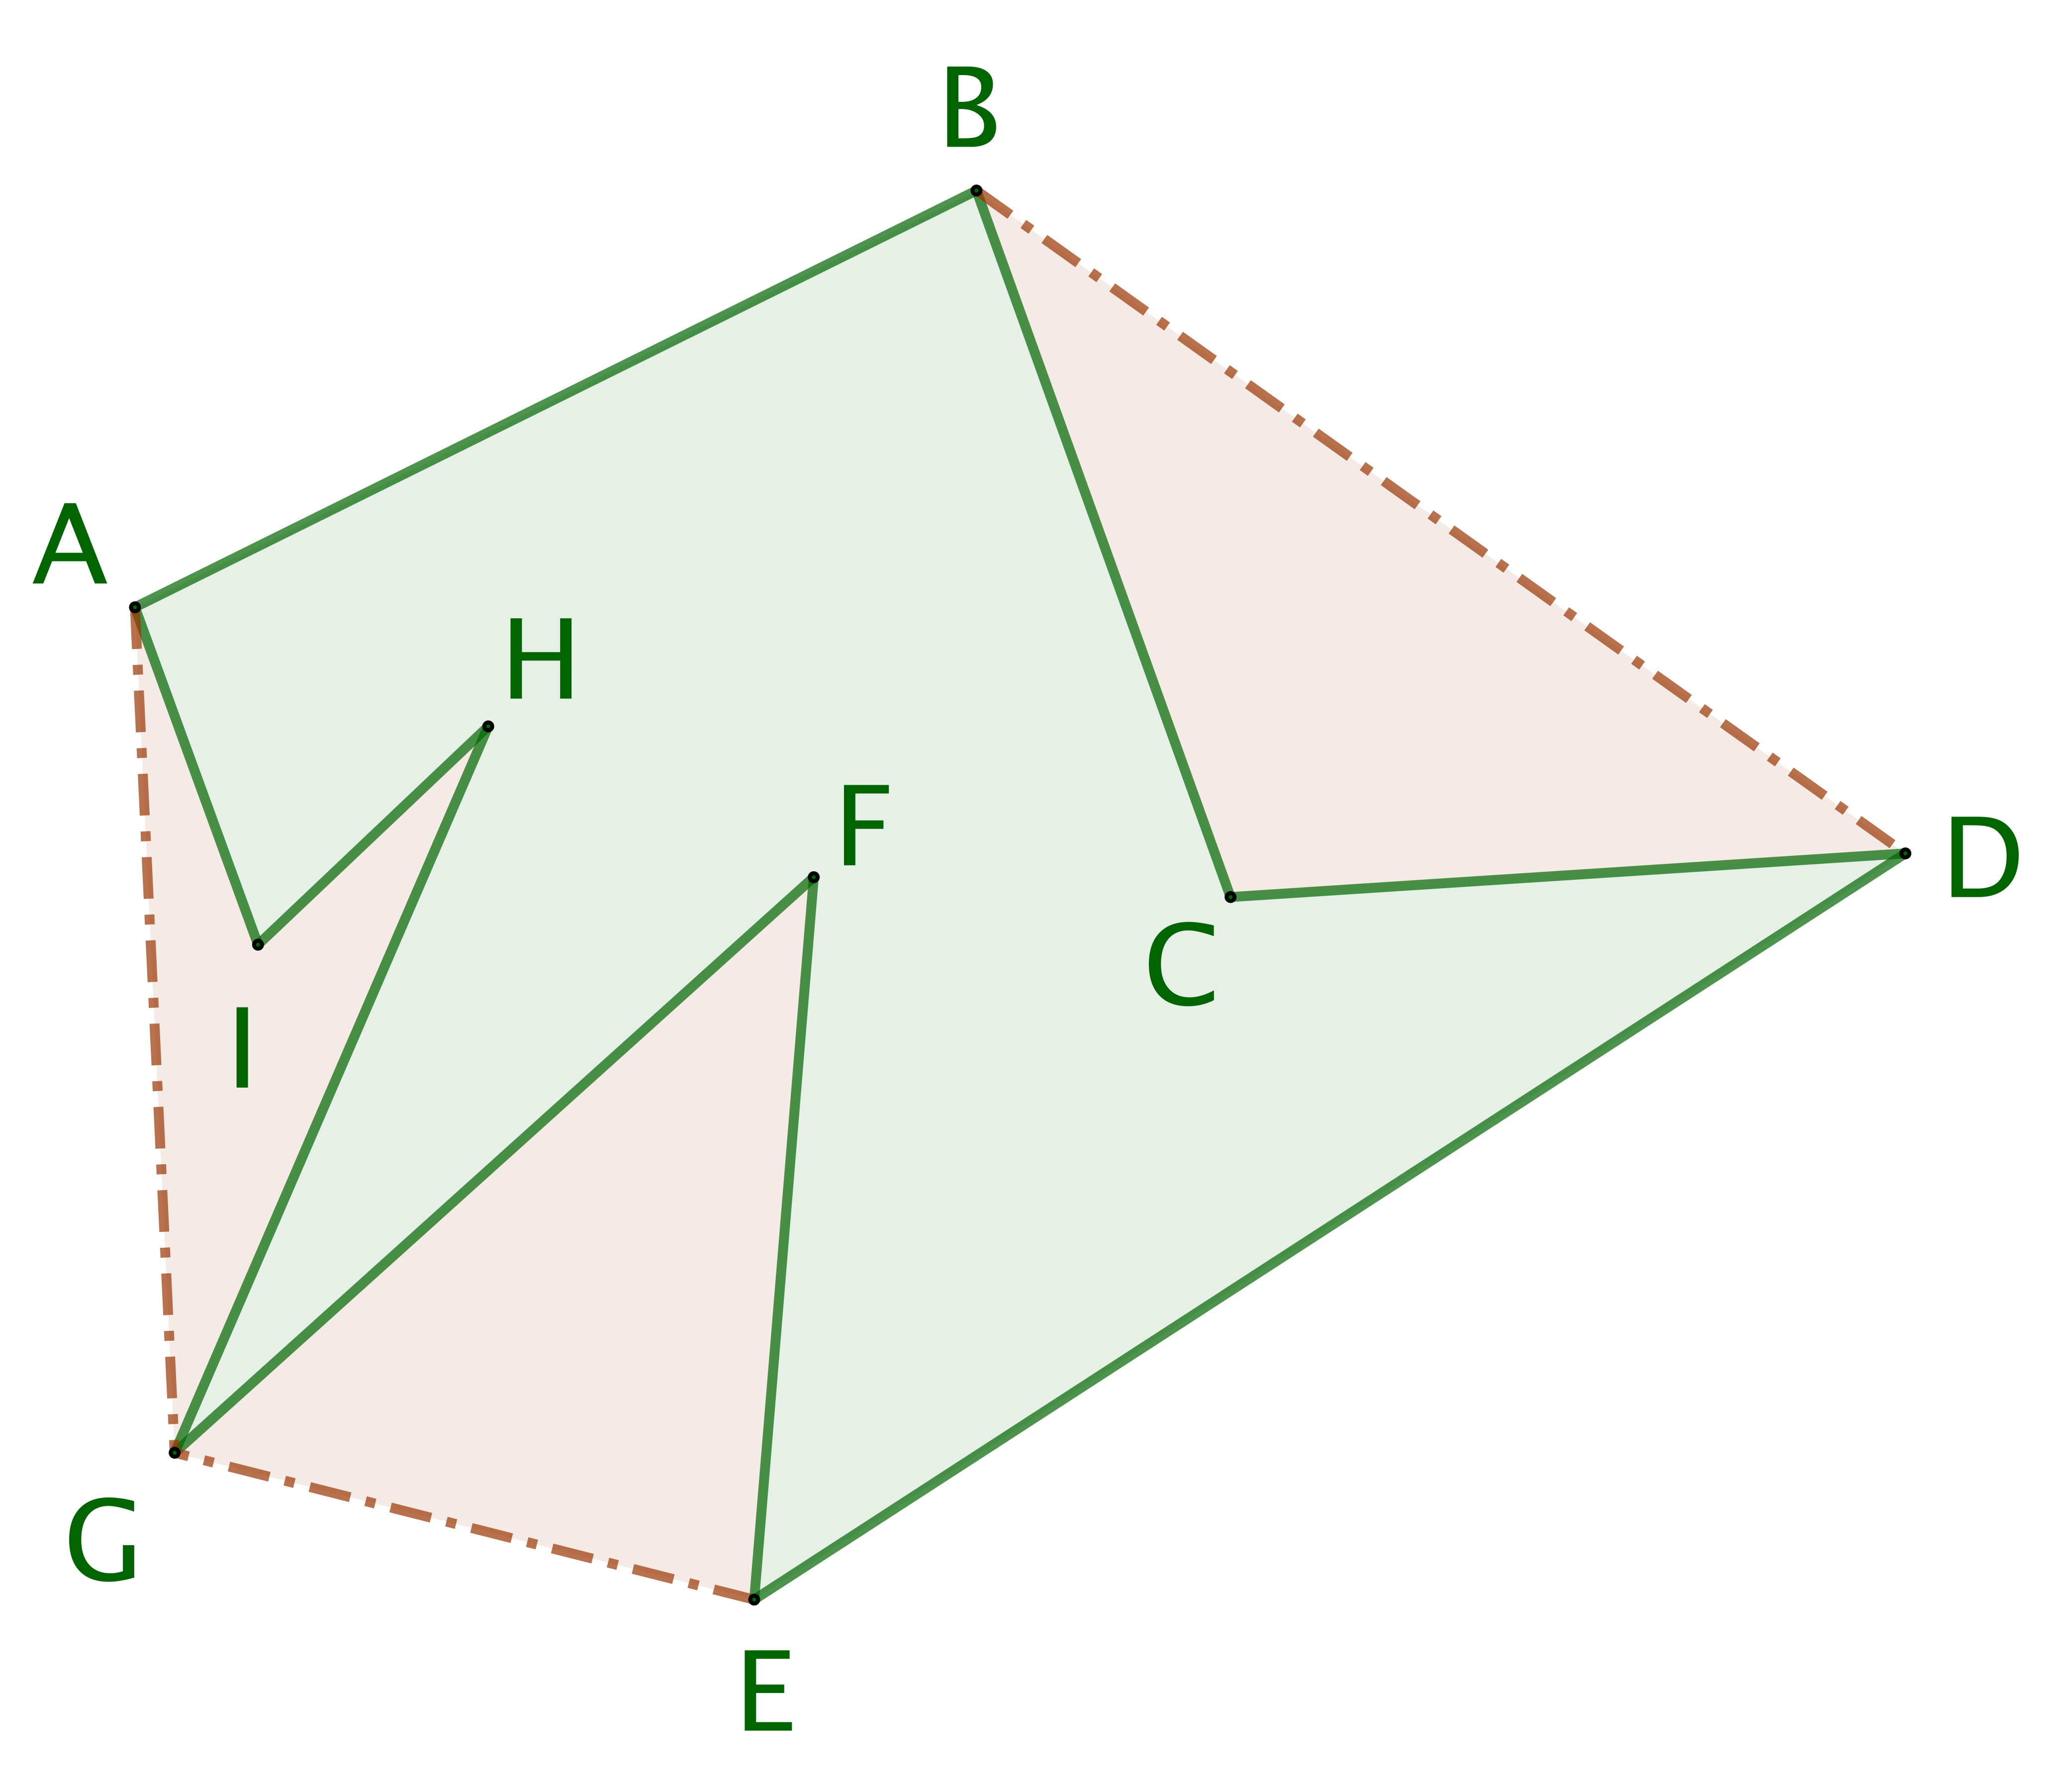
\includegraphics[scale=.4]{content/polygon/at-least-one/convex-hull.png}
%		
%		\smallskip
%		Exemple où $N = C$ et $O = B$.
%	\end{center}
%	
%		
%	Clairement, $\perim{\setproba{C}} < \perim{\setproba{L}}$.
%	Justifions que $\garea{\setproba{C}} > \garea{\setproba{L}}$ en reprenant les notations du fait \ref{ngone-trick} précédent.
%
%    \smallskip
%    
%    \noindent\kern-1.75ex
%    \begin{stepcalc}[style=ar*]
%		2 \garea{\setproba{L}} 
%	\explnext{}
%     	\abs*{\,
%    		\dsum_{j} \area{\setproba{L}_{2j + 1}}  -  \dsum_{j} \area{\setproba{L}_{2j}}
%	  	\,}
%	\explnext[\leq]{}
%     	  \dsum_{j} \area{\setproba{L}_{2j + 1}}  
%	    + \dsum_{j} \area{\setproba{L}_{2j}}
%	\explnext*[<]{$\setproba{L}$ n'est pas un \ngone\ convexe.}{}
%     	2 \area{\setproba{C}}
%	\explnext{}
%     	2 \garea{\setproba{C}}
%    \end{stepcalc}	
%	
%	\smallskip
%	
%	Il reste un problème à gérer: $\setproba{C}$ est un \kgone\ avec $k < n$. 
%	%
%	Une idée simple, formalisée après, est d'ajouter des sommets assez prêts des côtés de $\setproba{C}$ pour garder la convexité, une longueur strictement supérieure à $\perim{\setproba{L}}$, et une aire généralisée strictement plus grande que $\garea{\setproba{L}}$. Si c'est faisable, un agrandissement de rapport $r > 1$ donnera le \ngone\ $\setproba{P}$ cherché.
%	La figure suivante illustre cette idée.
%
%	\begin{center}
%		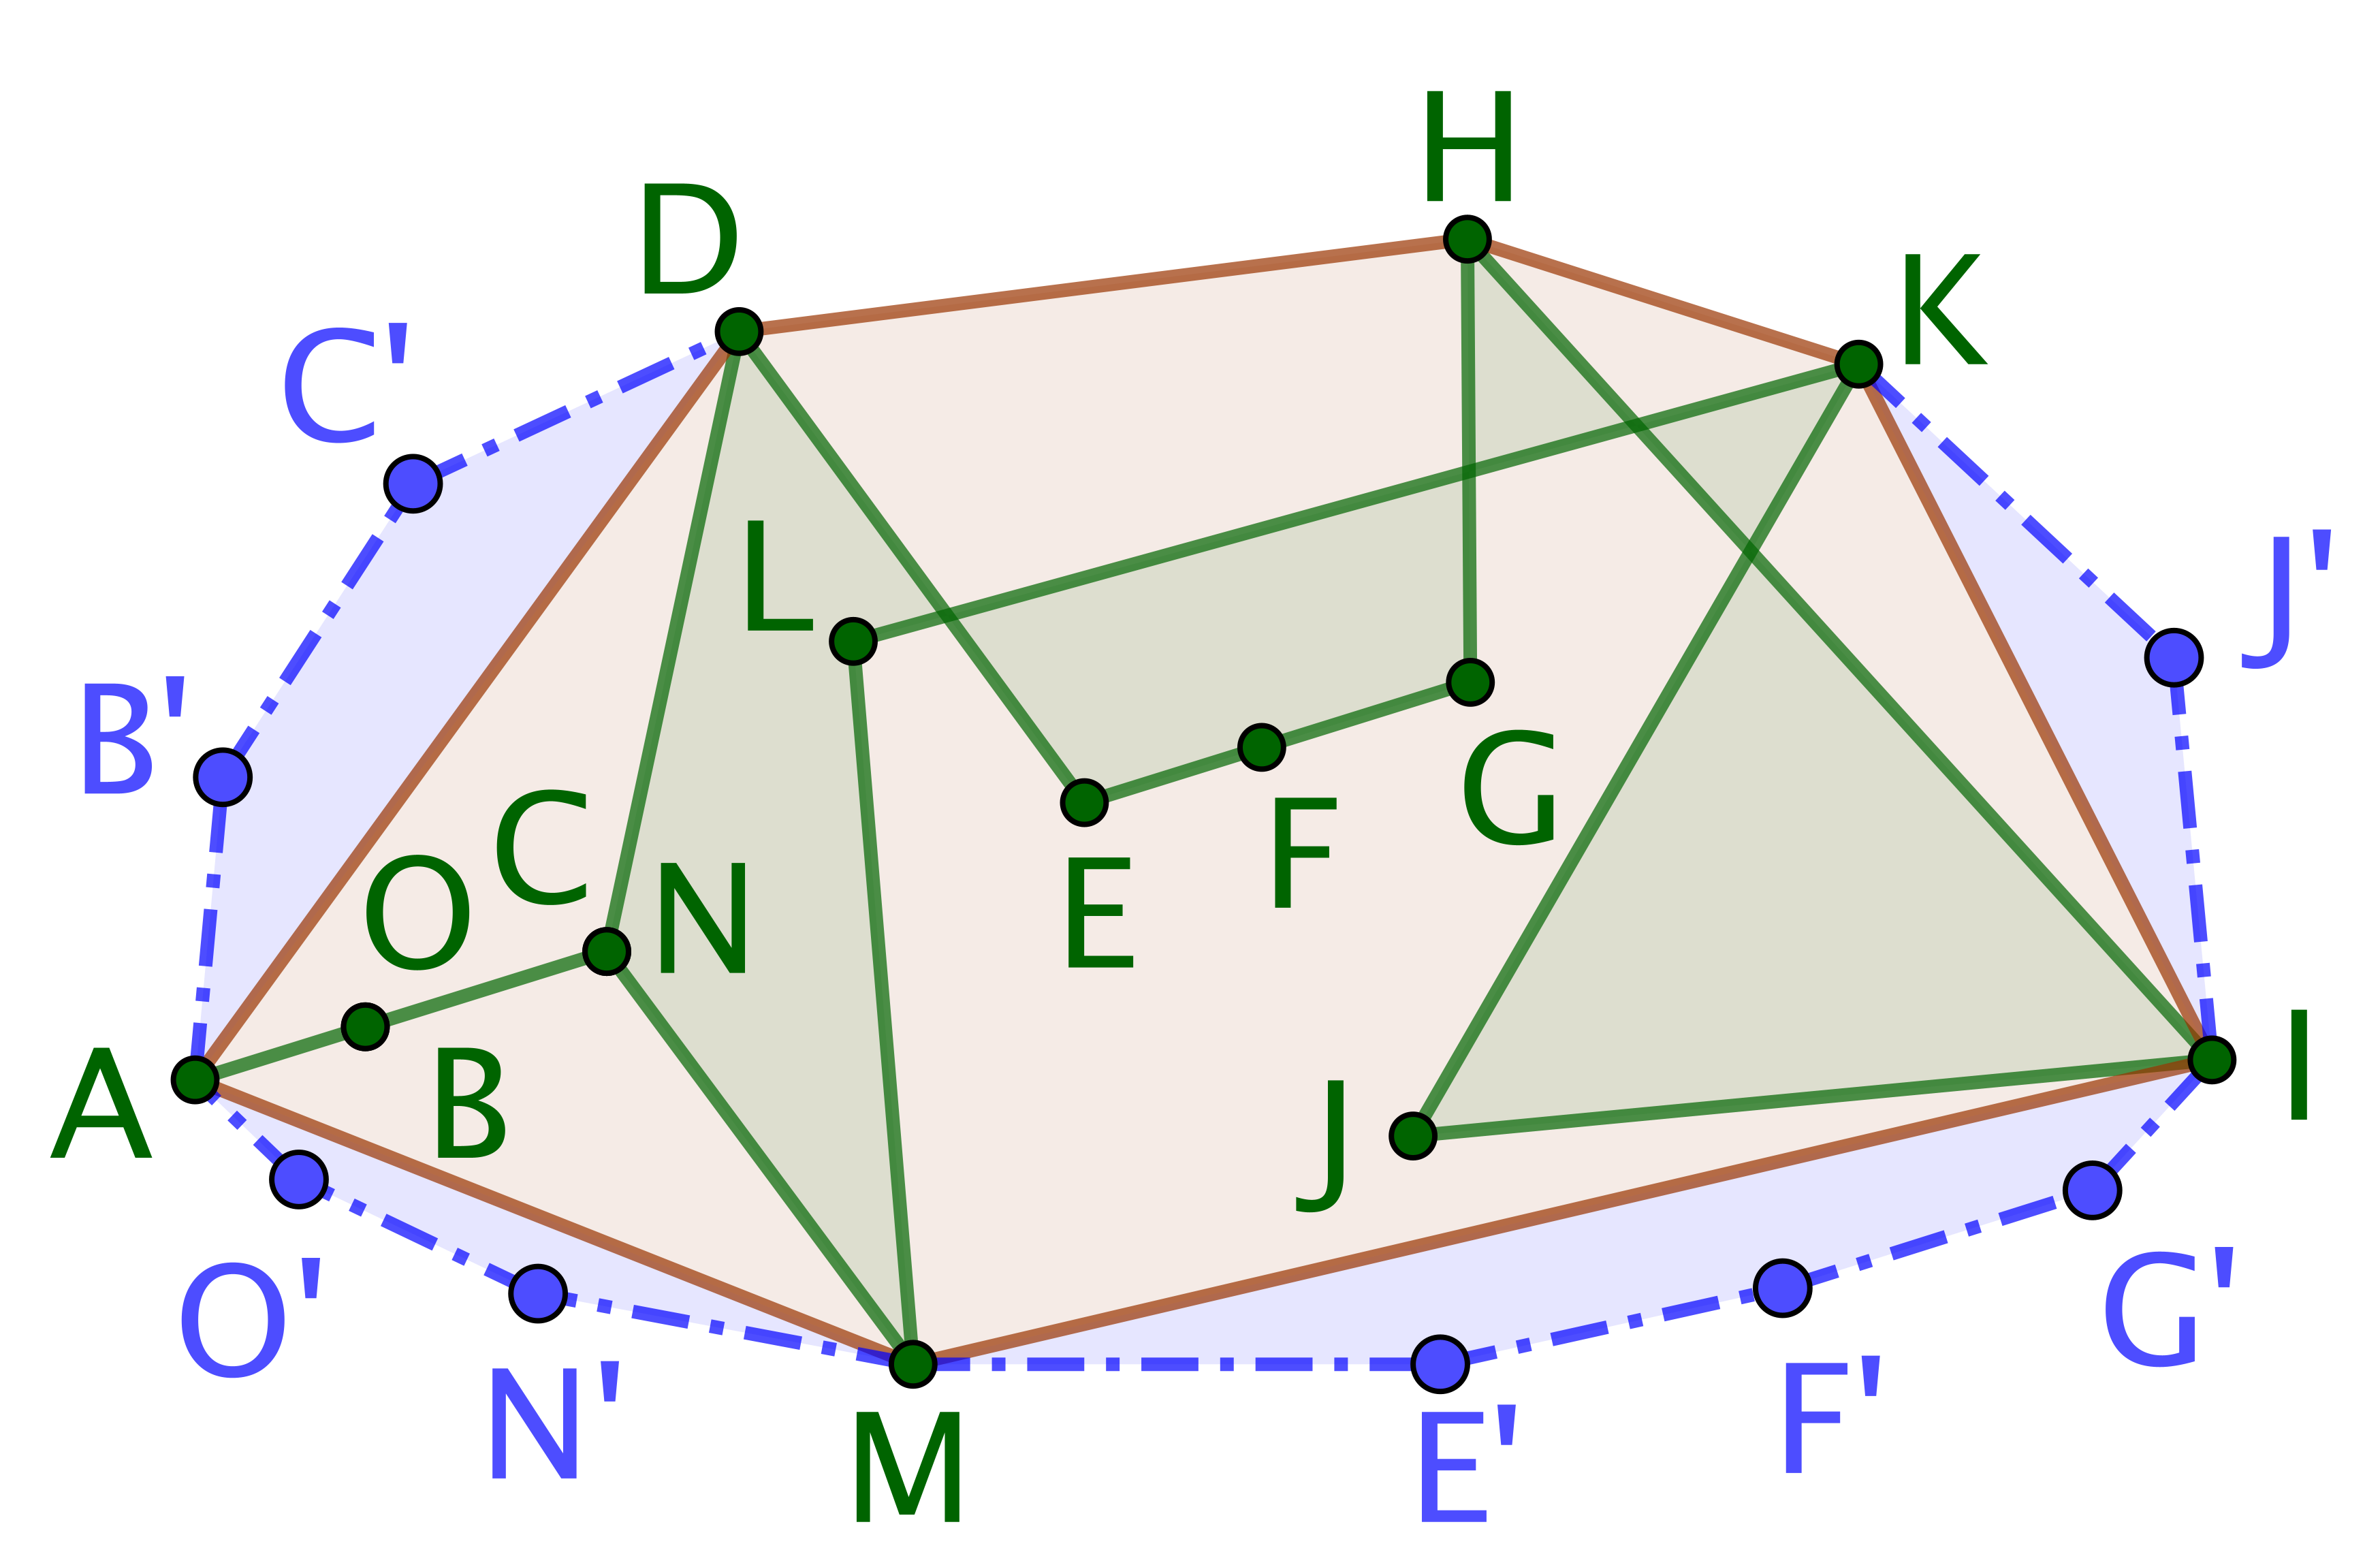
\includegraphics[scale=.4]{content/polygon/at-least-one/convex-hull-distortion.png}
%	\end{center}
%
%
%	Notons $s$ le nombre de sommets dans $\setproba{C}$, de sorte que $m = n - s$ compte les sommets manquants.
%	Si $m = 0$, il n'y a rien à faire.
%	Sinon, posons $\delta = \frac{\perim{\setproba{L}} - \perim{\setproba{C}}}{m}$.
%	%
%	\begin{enumerate}
%		\item \label{add-vertex-start}
%		Considérons $[AB]$ un côté quelconque de $\setproba{C}$.
%		Les droites portées par les côtés \og \emph{autour} \fg\ de $[AB]$ \og \emph{dessinent} \fg\ une région contenant toujours un triangle $ABC$ dont l'intérieur est à l'extérieur
%		\footnote{
%			C'est ce que l'on appelle de la \og \emph{low poetry} \fg\,.
%		}
%		de $\setproba{C}$ comme dans les deux cas ci-dessous.
%	%
%		\begin{multicols}{2}
%			\centering
%
%			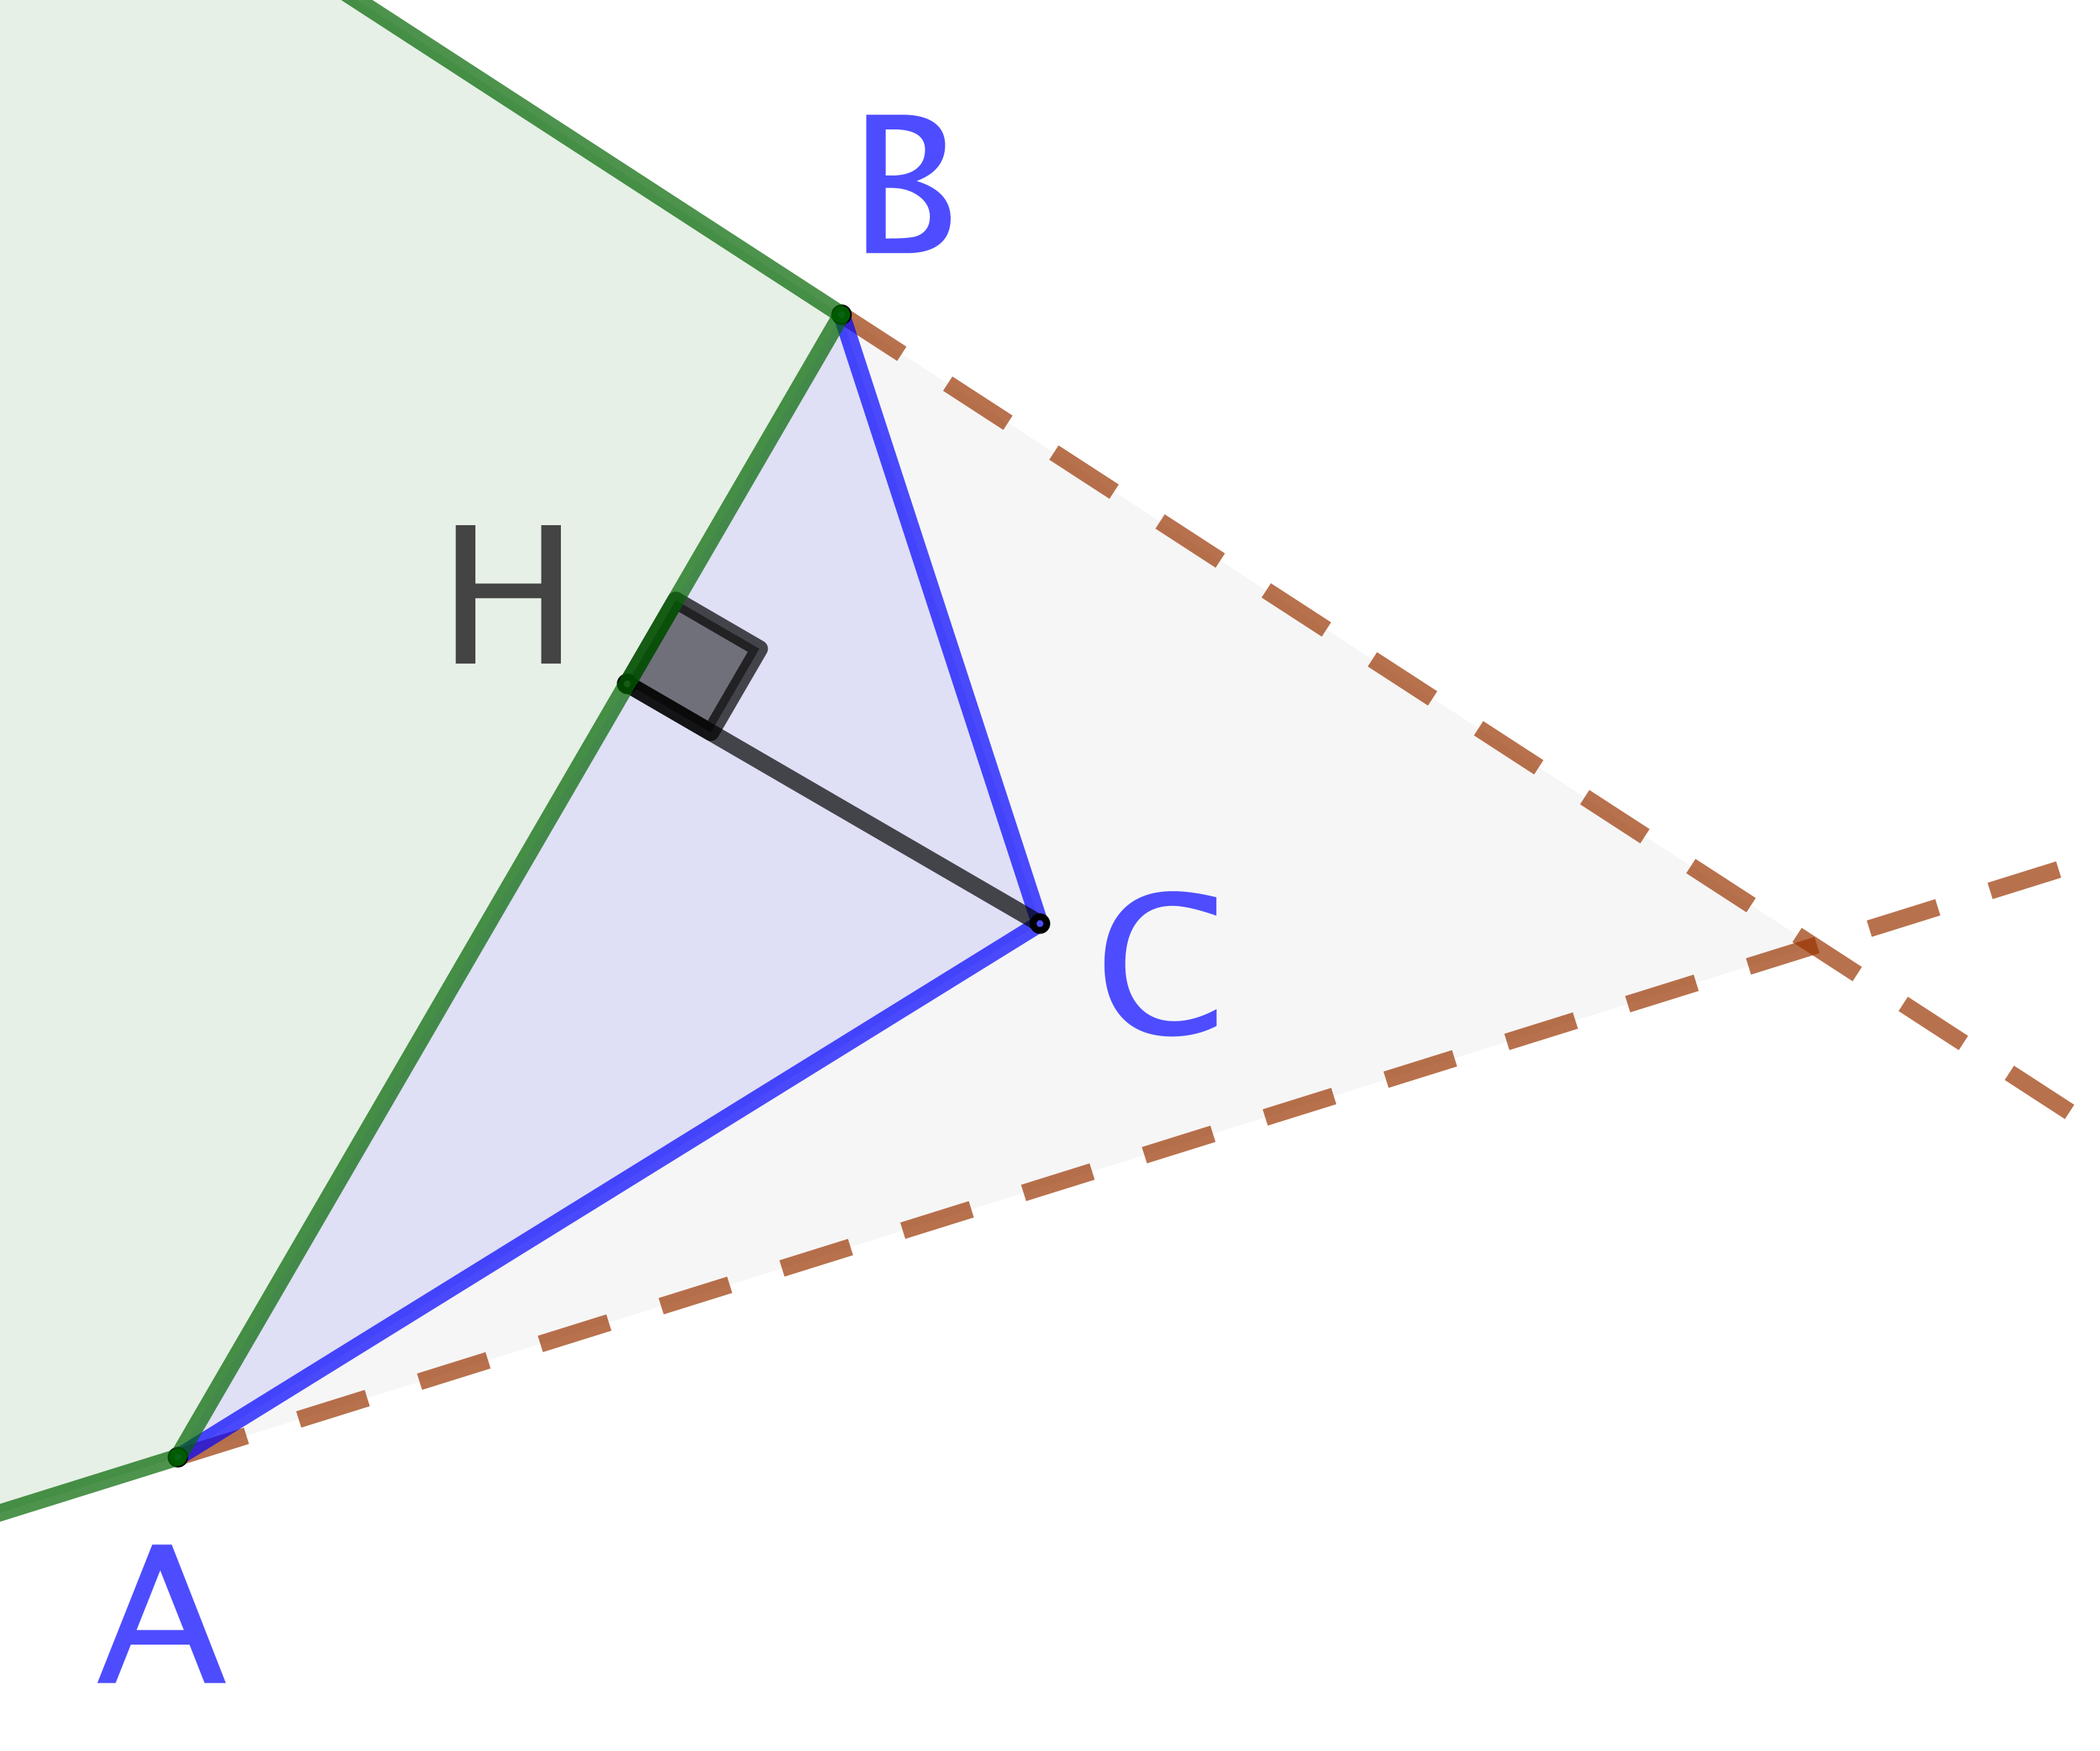
\includegraphics[scale=.4]{content/polygon/at-least-one/add-vertex-1.png}
%
%			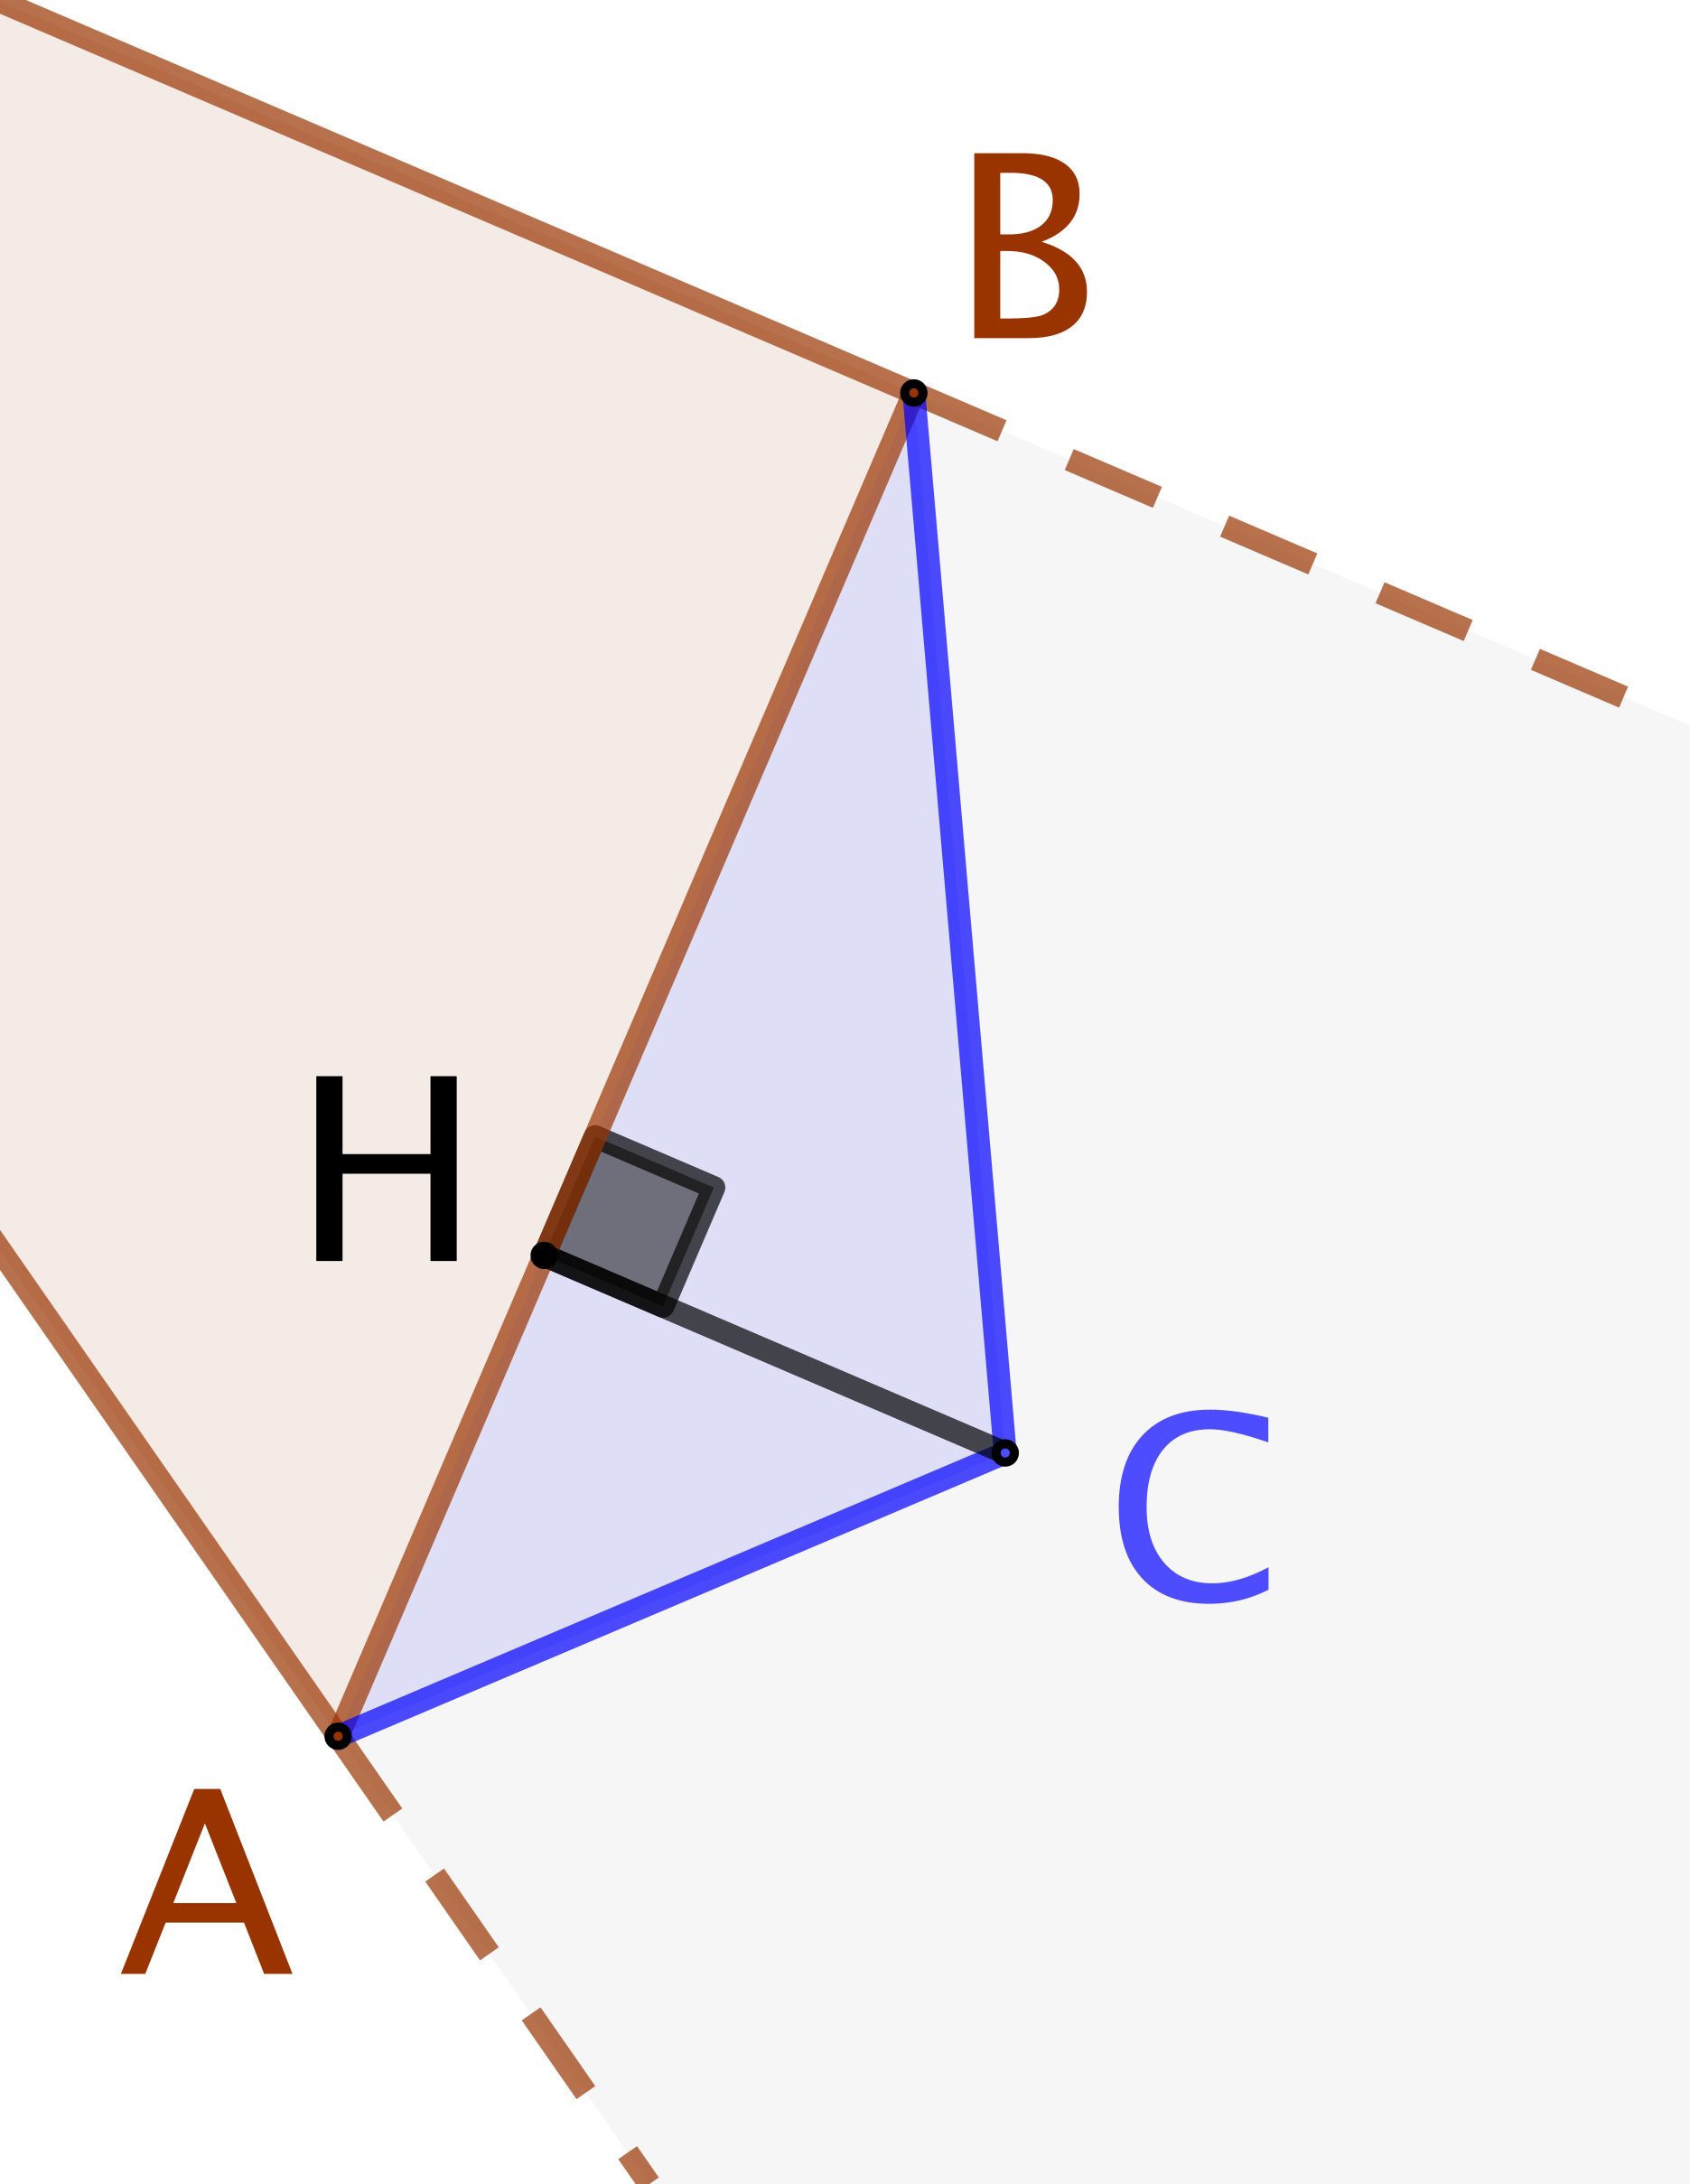
\includegraphics[scale=.4]{content/polygon/at-least-one/add-vertex-2.png}
%		\end{multicols}
%
%		\item Clairement, le polygone $\setproba{C}_+$ obtenu à partir de $\setproba{C}$ en remplaçant le côté $[AB]$ par les côtés $[AC]$ et $[CB]$ est un convexe avec un sommet de plus que $\setproba{C}$.
%
%		\item \label{add-vertex-end}
%		Comme $HC$ peut être rendu aussi proche de $0$ que souhaité, il est aisé de voir que l'on peut choisir cette distance de sorte que $AC + BC < AB + \delta$.
%		Dès lors, le périmètre de $\setproba{C}_+$ augmente inférieurement strictement à $\delta$ relativement à $\setproba{C}$.
%
%		\item En répétant $(m-1)$ fois les étapes \ref{add-vertex-start} à \ref{add-vertex-end}, nous obtenons un \ngone\ convexe $\setproba{C}^{\,\prime}$ tel que
%		$\garea{\setproba{C}^{\,\prime}} > \garea{\setproba{L}}$
%		et
%		$\perim{\setproba{C}^{\,\prime}} < \perim{\setproba{C}} + m \delta = \perim{\setproba{L}}$.
%	\end{enumerate}
%\end{proof}
%